\documentclass[11pt,a4paper]{article}

% Packages
\usepackage[utf8]{inputenc}
\usepackage[T1]{fontenc}
\usepackage{amsmath,amssymb}
\usepackage{graphicx}
\usepackage{float}
\usepackage{natbib}
\usepackage{doi}
\usepackage[margin=1in]{geometry}
\usepackage{setspace}
\usepackage{booktabs}
\usepackage{hyperref}
\usepackage{xcolor}
\usepackage{algorithm}
\usepackage{algpseudocode}
\usepackage{bbm}

% Revision highlighting (real-data extension): new or changed text in red
\newcommand{\rev}[1]{{\color{red}#1}}

% Citation style
\bibliographystyle{apalike}
\setcitestyle{authoryear,round,semicolon}

% Line spacing
\onehalfspacing

\title{Prediction Quality Versus Optimization Sophistication in Risk-Adjusted Clinical Scheduling}

% \author{%
%     \fontsize{10}{12}\selectfont
%     Alireza Moayedikia\textsuperscript{a,*} \and
%     Uffe Kock Wiil\textsuperscript{b} \and
%     Sara Fin\textsuperscript{c}
% }

% \date{%
%     \fontsize{10}{12}\selectfont
%     \textsuperscript{a}School of Business and Entrepreneurship, Swinburne University of Technology, Melbourne, Australia \\
%     \textsuperscript{b}The Maersk Mc-Kinney M{\o}ller Institute, University of Southern Denmark, Odense, Denmark \\
%     \textsuperscript{c}Australian Regenerative Medicine Institute, Monash University, Melbourne, Australia \\[2pt]
% }

\date{}

\begin{document}
\sloppy
\maketitle

% \renewcommand{\thefootnote}{*}
% \footnotetext{Corresponding author: Alireza Moayedikia is with the department of Business Technology and Entreprenourship, Swinburne University of Technology, John Street, Hawthorn 3122 VIC Australia. Email: amoayedikia@swin.edu.au}
% \renewcommand{\thefootnote}{\arabic{footnote}}

\begin{abstract}
Clinical trials require precise coordination of diagnostic procedures, yet conventional scheduling systems treat patients as interchangeable, ignoring observable heterogeneity in procedure completion risk. We investigate where operational value resides in prescriptive analytics systems that integrate machine learning prediction with stochastic optimization. Using Alzheimer's disease clinical trials as a structurally demanding test case, we design a data architecture grounded in standardized clinical assessments and train gradient boosting models on simulation-augmented patient cohorts---with clinical profiles and failure rates calibrated to published findings---to estimate patient-specific Magnetic Resonance Imaging scan failure probabilities, then embed these predictions as Bernoulli service time distributions in a stochastic job-shop scheduling formulation. Computational experiments reveal a striking inversion of conventional priorities: prediction quality, not optimization sophistication, drives scheduling performance. A simple risk-first sequencing heuristic achieves statistically indistinguishable performance from mixed-integer programming, reducing overtime probability by approximately nine percentage points compared to age-based stratification, despite requiring negligible computation time. Notably, applying machine learning to demographic features alone provides no advantage over simple stratification rules, demonstrating that value derives from incorporating cognitive and behavioral biomarkers rather than from model complexity. A counter-intuitive finding emerges: age-based heuristics, embodying common clinical intuition, underperform schedules that ignore patient heterogeneity entirely, because partial information introduces systematic misallocation. The framework exhibits robustness to prediction error and provides increasing benefit for higher-risk patient populations. \rev{All experiments are additionally replicated on a second evaluation arm in which patient cohorts are sampled from real participant records of the National Alzheimer\'s Coordinating Center: every qualitative finding is preserved, and the advantage of full-feature prediction over age-based stratification nearly doubles, to 17.5 percentage points. Predicted risk also significantly discriminates real scan-quality degradation recorded by NACC\'s neuroimaging quality-control pipeline, with cognitive screening---not age---carrying the signal.} For the AD/MRI scheduling case studied here, these findings suggest that facilities should prioritize investment in predictive infrastructure over optimization software; whether this priority extends to other capacity-constrained diagnostic settings remains an empirical question for future cross-domain replication.
\end{abstract}

\noindent\textbf{Keywords:} Scheduling; Stochastic programming; Prescriptive analytics; Machine learning; Healthcare operations



\newpage
\section{Introduction}
\label{sec:introduction}

Operational scheduling in healthcare routinely ignores patient-level heterogeneity: clinical assessments capture individual risk factors that demonstrably affect procedure outcomes \citep{porembka2025disparities}, yet appointment systems assign uniform time slots regardless of individual completion probabilities. The resulting cascading delays, staff overtime, and resource underutilization represent a gap between predictive information and prescriptive action that the emerging prescriptive analytics paradigm \citep{bertsimas2020predictive, elmachtoub2022smart} has only begun to address---particularly in settings requiring stochastic formulations that capture outcome variance rather than expected-value approximations \citep{sadana2025contextual}. We develop a two-phase prescriptive analytics framework that integrates machine learning prediction with stochastic optimization for appointment scheduling in capacity-constrained diagnostic services, grounded in the operationally demanding context of MRI neuroimaging within Alzheimer's disease clinical trials. This application domain presents the scheduling challenge in acute form: the very pathology under investigation (progressive neurodegeneration affecting attention, executive function, and motor control) elevates scan failure probability, yet standardized research protocols preclude the ad hoc schedule adjustments that might accommodate such heterogeneity in routine clinical practice.

Phase III Alzheimer's disease trials routinely enroll thousands of participants across dozens of international sites, with per-patient costs exceeding \$40,000 and total program expenditures frequently surpassing \$2 billion \citep{cummings2014clinical}. These trials demand multi-modal data collection combining standardized cognitive assessments, structural and functional MRI neuroimaging, and cerebrospinal fluid biomarker sampling---procedures that must occur within protocol-specified visit windows to maintain data integrity and regulatory compliance. When an MRI scan fails due to excessive patient motion and must be repeated, consequences cascade throughout the daily schedule: subsequent patients experience extended waiting times, staff incur overtime costs, and the facility's effective throughput diminishes. Empirical evidence indicates that this is not a marginal operational concern. \citet{andre2015quantifying}, in a foundational analysis of clinical MR examinations at a level-I trauma center, documented that motion artifacts necessitated repeat sequences in 19.8\% of all examinations, generating an estimated \$115{,}000 per scanner per year in foregone revenue (sensitivity range \$92{,}600--\$139{,}000) and approximately \$592 per hour in lost throughput. The burden falls disproportionately on patients with reduced capacity to remain still: prevalence of significant motion artifacts rises from 7.5\% in outpatient examinations to 29.4\% among inpatient and emergency department populations \citep{andre2015quantifying}, and a multivariate analysis of 775 brain MRI scans recently identified advancing age and motor symptoms as independent predictors of motion contamination \citep{krag2025motion}. In cohorts with established cognitive impairment---precisely the population that Alzheimer's trials are designed to study---published estimates of MRI scan failure rates range from 10\% to 30\% \citep{porembka2025disparities}, an order of magnitude above what is observed in well-managed research settings with extensive pre-screening.

A 72-year-old participant with moderate cognitive impairment and no prior scanning history faces categorically different operational risk than a 65-year-old with normal cognition who has successfully completed multiple research scans, yet current scheduling systems treat these patients identically.


Healthcare scheduling has been a central topic in operations research since the foundational reviews of \citet{cayirli2003outpatient} and \citet{gupta2008appointment}, with recent surveys \citep{ahmadi2017outpatient, youn2022planning, belien2025fifty} confirming its enduring importance and persistent translation gaps. The canonical two-stage stochastic program of \citet{denton2003sequential} minimizes a weighted combination of expected patient waiting time, provider idle time, and overtime costs, with first-stage appointment time decisions and second-stage recourse capturing realized outcomes. This formulation has spawned extensive methodological development: sample average approximation with established convergence properties \citep{kleywegt2002sample, mancilla2012sample}, parallel-resource extensions \citep{denton2010optimal}, multi-stage progressive hedging for surgical scheduling \citep{gul2015progressive}, and recent emergency department staffing applications \citep{marchesi2025stochastic}. A common limitation runs through this literature: service-time distributions are parameterized at the procedure-type level, estimated from population-level historical data. \citet{denton2007optimization} demonstrated that scheduling high-variance procedures later in the day substantially reduces expected overtime costs, but the variance in question is procedure-type-specific, not patient-specific. Even sophisticated contributions on multi-disciplinary clinic planning \citep{leeftink2019stochastic}, patient unpunctuality \citep{jiang2019stochastic}, and robust surgical scheduling \citep{neyshabouri2017two} maintain this aggregation level. Distributionally robust optimization has emerged when distributions are imprecisely known \citep{jiang2017integer, shehadeh2021distributionally}, but these approaches construct ambiguity sets from population data rather than patient covariates. MRI and diagnostic imaging scheduling has received comparatively limited attention \citep{qiu2019mri, sun2021stochastic, bouguerra2023integrating}, with patient-specific conditioning entirely absent. \citet{silvaaravena2025mri} recently applied digital twins and reinforcement learning to MRI scheduling, modeling machine failures as Bernoulli events, but failure probabilities were specified exogenously rather than predicted from patient characteristics. The job-shop scheduling analogy for clinical workflows appears in \citet{burdett2018flexible} and \citet{pham2008surgical} without patient-heterogeneous processing times.


Clinical ML has achieved high accuracy across image quality assessment, no-show prediction, Alzheimer's biomarker analytics, and procedure duration forecasting, yet a consistent pattern emerges: models terminate at prediction without translation into operational decisions \citep{kelly2019key, seneviratne2020bridging}. In MRI quality assessment, \citet{esteban2017mriqc} introduced MRIQC using random forests on engineered image quality metrics, with subsequent deep-learning approaches achieving 91--96\% accuracy in motion artifact detection \citep{vakli2023automatic, beljaards2024motion}; however, these tools operate post-acquisition rather than predicting scan failure prospectively. The closest approach to pre-scan prediction appears in \citet{porembka2025disparities}, who identified demographic and clinical predictors of motion artifacts across 68{,}000 MRI examinations with odds ratios of 1.5--3.3 and significant nonlinear interactions, explicitly recommending scheduling adjustments but without constructing a predictive model or optimization method. Patient no-show prediction represents the most developed predict-to-schedule pipeline \citep{dantas2018noshows, asan2022pediatric, silva2023decision}, with \citet{samorani2021overbooked} bridging prediction and operations via fairness-constrained scheduling---though for overbooking levels rather than service-time distributions. The Alzheimer's ML literature provides a clinical foundation but targets endpoint prediction rather than operational outcomes: \citet{song2023random} achieved 90.8\% concordance on NACC data, \citet{elsappagh2024explainable} achieved 98.9\% F1 scores with interpretable models, and \citet{coupe2019mri} showed that combining MRI biomarkers with cognitive scores improves prediction over either modality alone. Crucially, the NACC dataset has never been repurposed for operational prediction despite containing precisely the clinical variables that would inform scan failure risk. Procedure duration prediction has gained traction in surgical contexts \citep{bartek2019improving, master2023multicenter, spence2023scoping, martinez2021machine}, establishing feasibility but without analogues for MRI failure prediction in cognitively impaired populations.


Three seminal contributions anchor the prediction--optimization integration literature. \citet{elmachtoub2022smart} introduced Smart Predict-then-Optimize (SPO) with decision-error loss functions enabling end-to-end training through optimization layers. \citet{bertsimas2020predictive} developed prescriptive analytics via ML methods for conditional stochastic optimization, demonstrating substantial gains over sample average approximation. \citet{ban2019big} proved that omitting available covariate features yields statistically inconsistent data-driven decisions---a theoretical result directly motivating our use of patient characteristics in scheduling. The comprehensive survey of \citet{sadana2025contextual} catalogued contextual stochastic optimization across decision rule, sequential predict-then-optimize, and integrated end-to-end paradigms, explicitly identifying healthcare as an underexplored domain, while \citet{deng2022predictive} formalized ``Predictive Stochastic Programming'' with statistical foundations for feeding ML-estimated conditional distributions into stochastic programs. Within healthcare, the integration landscape reveals progression toward but not yet achieving full stochastic formulations with patient-specific distributional parameters. \citet{srinivas2018prescriptive} pioneered ML-driven outpatient scheduling but used heuristic rules rather than mathematical programming. \citet{salah2022predict} advanced to a predict-then-schedule framework, achieving over 50\% waiting-time reduction in simulation but acknowledging that ``inputting predicted values directly into the optimization model may result in sub-optimal decisions when the model objective is nonlinear in predicted parameters.'' \citet{olya2022integrated} proposed deep multi-task learning feeding into two-stage stochastic optimization for chronic disease resource management but focused on aggregate capacity planning rather than individual scheduling. The most directly analogous works are \citet{gower2025predict}, who used neural-network duration predictions for surgical scheduling but as point estimates in deterministic optimization, and \citet{rottmann2025case}, who applied quantile regression forests to surgical planning and achieved 35\% cost improvement by capturing distributional information beyond point predictions---methodologically closest to our approach but in surgical rather than imaging contexts. End-to-end approaches face significant computational challenges when the optimization involves integer variables or recourse structures \citep{mandi2024decision}---precisely the characteristics of stochastic healthcare scheduling.

Our framework addresses these gaps through a sequential two-phase architecture whose contribution lies not in the sequential design per se, but in the principled interface between phases: rather than feeding point predictions into deterministic optimization with procedure-level parameters \citep{salah2022predict}, we use ML-predicted failure probabilities to parameterize patient-specific service-time distributions that preserve outcome variance within a computationally tractable formulation.

This paper develops a two-phase prescriptive analytics framework for MRI appointment scheduling in Alzheimer's disease clinical trials, designed to answer a focused operational question: \textit{when patient cognitive and behavioral characteristics predict scan failure risk, does the primary operational benefit derive from better prediction or better optimization?} We deliberately ground both the framework and the question in this specific clinical context; the broader implications for any predict-then-optimize setting with observable individual heterogeneity in service outcomes are revisited in Section~\ref{sec:discussion}.

In Phase 1, we train machine learning models on simulation-augmented patient cohorts whose cognitive, behavioral, and clinical profiles are calibrated to published Alzheimer's disease population characteristics, predicting each patient's individualized probability of MRI scan failure, denoted $p_i$ for patient $i$. Critically, we use these predicted probabilities not as point estimates for expected-value scheduling, but as parameters defining patient-specific Bernoulli outcome distributions.

In Phase 2, we formulate a stochastic mixed-integer program where patient-specific service time distributions are parameterized by these ML-predicted probabilities. For patient $i$, the service time follows a Bernoulli-weighted mixture: the nominal scan duration $d_i^0$ with probability $(1-p_i)$ or the extended duration $d_i^0 + \delta_i$ (accounting for repositioning, rescanning, or session termination) with probability $p_i$. Following computational tractability arguments established by \citet{denton2003sequential} and \citet{mancilla2012sample}, we implement an expected-value formulation where risk-adjusted durations $\tilde{d}_i = d_i^0 + p_i \cdot \delta_i$ allocate buffer time proportionally to predicted failure probability. This formulation captures patient-specific risk heterogeneity while maintaining the computational efficiency required for real-time operational deployment.

By systematically varying the prediction source (no prediction, age-only rules, age-only ML, full ML with cognitive and behavioral features) and the optimization method (heuristic sorting rules, mixed-integer programming) across comprehensive computational experiments, we establish three empirical findings for the Alzheimer's MRI scheduling case.

First, \textit{prediction dominates optimization for this problem class}. A simple longest-processing-time heuristic achieves statistically indistinguishable performance from a Stochastic-MILP formulation, despite the latter requiring $35{,}000\times$ more computation time at $n = 10$ patients---a gap that widens to complete intractability at realistic clinic volumes ($n \geq 20$), where the MILP fails to find optimal solutions within practical time limits while LPT solves in constant time. In this case, where the optimization structure admits a near-optimal risk-first priority rule, investment in better prediction yields far greater returns than investment in better optimization.

Second, \textit{feature richness dominates model complexity}. Applying gradient boosting to age-derived features alone provides no advantage over simple age-bracket rules. The value of machine learning emerges only when the feature set includes cognitive assessments and behavioral symptoms---approximately 80\% of predictive signal resides in non-demographic features. For the AD/MRI case studied here, the bottleneck to effective prescriptive analytics is therefore data infrastructure rather than algorithmic sophistication: collecting and integrating the right features matters more than choosing the right model.

Third, \textit{partial information can be worse than no information}. Age-based heuristics, which embody a common form of clinical domain knowledge, actually underperform deterministic scheduling that ignores patient heterogeneity entirely. This counter-intuitive result arises because age is a weak proxy for procedural failure risk, and scheduling based on an inadequate proxy introduces systematic misallocation that uniform treatment avoids. The mechanism is general---a weak proxy used confidently is worse than no proxy used at all---but whether the same inversion arises in other settings where practitioners apply intuitive risk stratification depends on the specific proxy and the underlying risk structure, and would require dedicated empirical investigation.

\rev{All three findings are established on simulation-augmented cohorts and then re-established on a second evaluation arm in which cohorts are sampled from real participant records of the National Alzheimer's Coordinating Center (NACC) Uniform Data Set (Section~\ref{sec:real_data_arm}). Every qualitative pattern replicates, and the penalty for age-based scheduling nearly doubles on real covariates---evidence that the simulation-augmented experiments, if anything, understate the first two findings. A further validation (Section~\ref{sec:qc_validation}) links predicted risk to real, independently recorded MRI quality outcomes: predicted high-risk participants have significantly more motion-flagged studies, and cognitive screening out-discriminates age---real-outcome support for the mechanism behind the second and third findings.}

The framework architecture is, by construction, transferable to any capacity-constrained service system where observable individual characteristics predict processing outcomes---oncology treatment centers where comorbidities affect infusion tolerance, surgical preparation units where anxiety indicators predict sedation requirements, or manufacturing cells where product specifications predict processing complexity. We emphasize, however, that this transferability is structural rather than empirically demonstrated: the experimental results in this paper are specific to the AD/MRI case. The Alzheimer's trial serves as a deliberate first test case because patient heterogeneity is clinically documented and measurable through standardized cognitive assessments, yet operationally ignored by current trial management systems---making it a setting where the framework's data-infrastructure prerequisites are plausibly satisfied. Section~\ref{sec:discussion} returns to what would be required to establish cross-domain transferability empirically.

The remainder of this paper proceeds as follows. Section~2 develops the method, including the data architecture, predictive model, and stochastic scheduling formulation. Section~3 presents computational experiments on simulation-augmented test instances\rev{, together with a replication of every experiment on cohorts sampled from real NACC participant records (Section~\ref{sec:real_data_arm})}. Section~4 discusses theoretical and practical implications, and Section~5 concludes. Figure~\ref{fig:framework} illustrates the two-phase architecture.

% FIGURE 1: Framework (place at end of Introduction)
\begin{figure}[H]
    \centering
    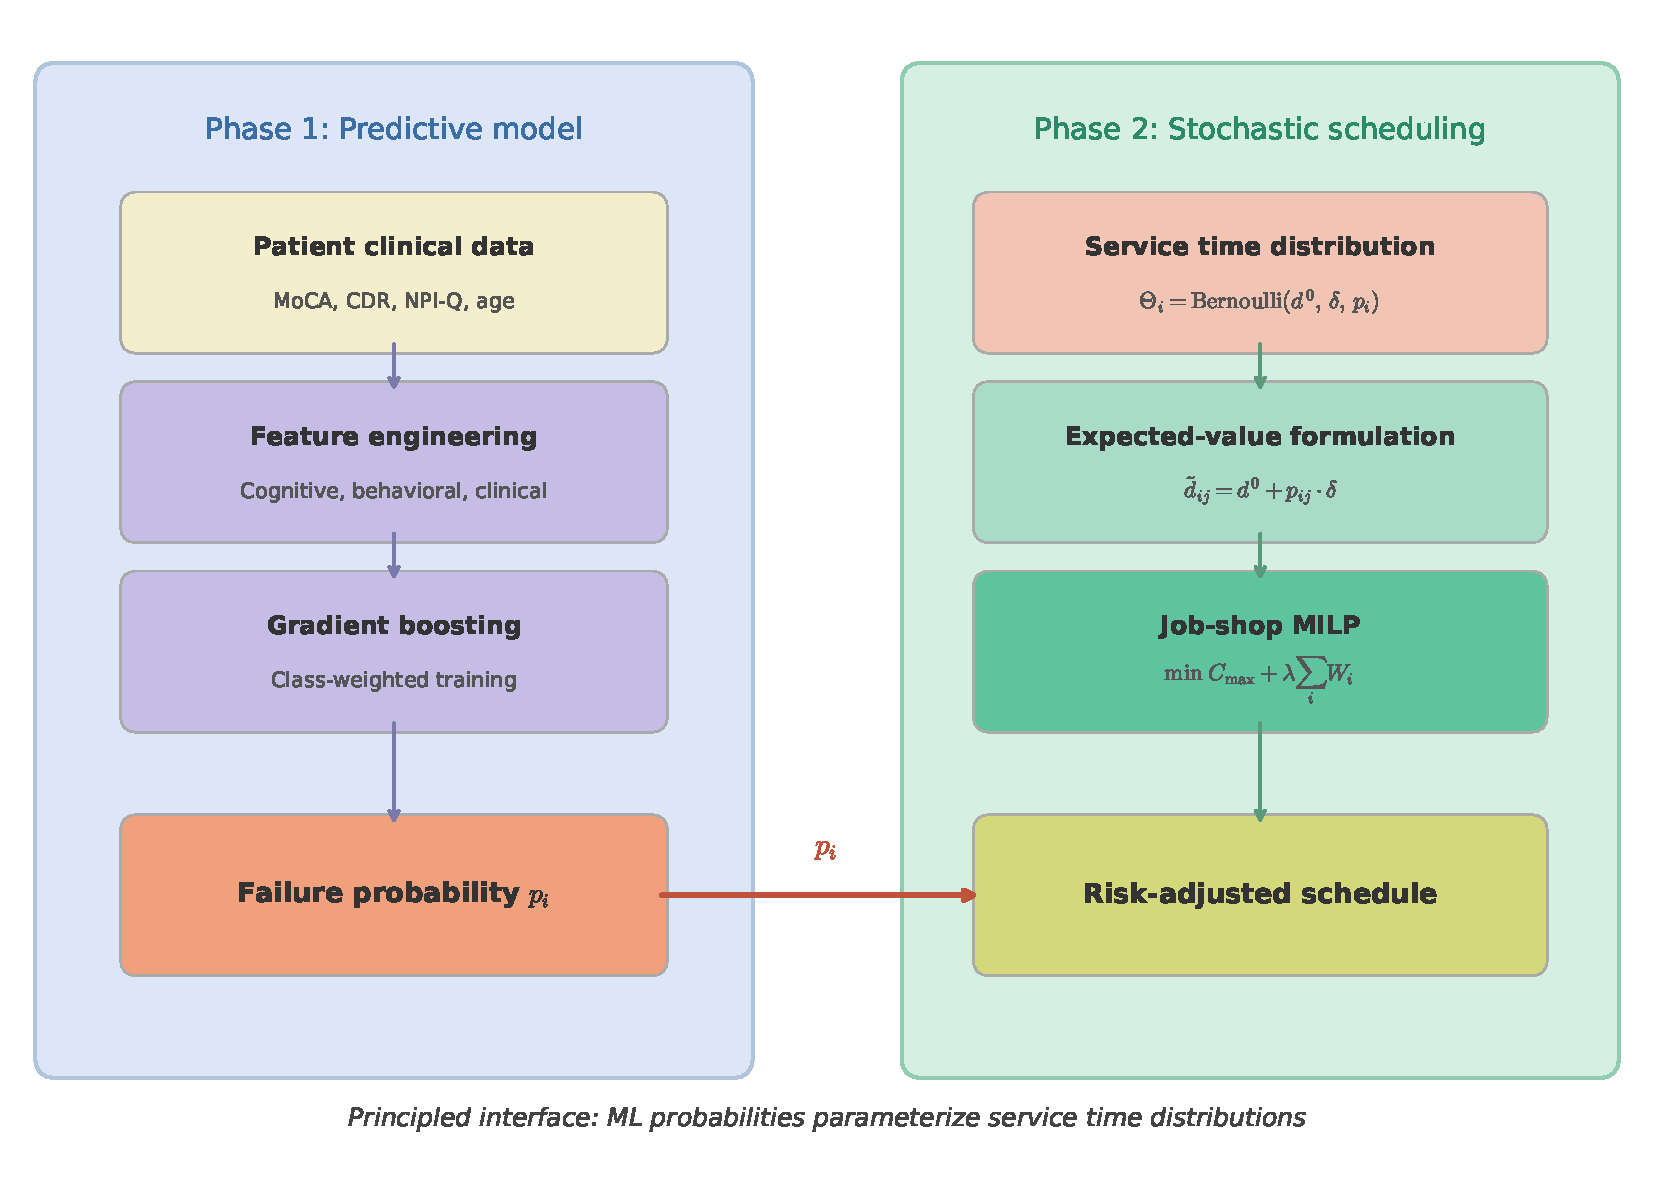
\includegraphics[width=\textwidth]{fig_framework.pdf}
    \caption{Two-phase prescriptive analytics framework. The architectural elements---feature engineering pipeline, gradient-boosting risk classifier, Bernoulli service-time distribution, expected-value reformulation, and job-shop MILP---are domain-agnostic and reusable across capacity-constrained service systems with observable individual heterogeneity. The Phase~1 input layer (MoCA, CDR, NPI-Q, age) is case-specific to Alzheimer's disease clinical trials; transferring the framework to another setting requires substituting domain-appropriate covariates predictive of service-outcome variability (e.g., comorbidity indices for oncology infusion scheduling, anxiety screening scores for pediatric MRI). The interface mechanism by which ML-predicted probabilities parameterize patient-specific service-time distributions is preserved across domains.}
    \label{fig:framework}
\end{figure}


\newpage
\section{Method}

This section develops the three components of our prescriptive analytics framework, expanding the two-phase architecture introduced in Figure~\ref{fig:framework}. Phase~1 (the predictive model) is treated in two subsections because its data architecture warrants separate exposition: Section~\ref{sec:data_architecture} describes the data architecture that temporally aligns asynchronous clinical and imaging records, validated on the National Alzheimer's Coordinating Center (NACC) Uniform Data Set, and explains the simulation-augmented cohort design used for model training and evaluation; Section~\ref{sec:predictive_model} then presents the feature engineering pipeline and gradient boosting model that transforms cognitive, behavioral, and clinical biomarkers into patient-specific failure probabilities $p_i$. Phase~2 (the stochastic scheduling component) is treated in Section~\ref{sec:scheduling_formulation}, which formulates the stochastic job-shop scheduling problem in which these ML-predicted probabilities parameterize Bernoulli service-time distributions, and derives the expected-value approximation used for computational tractability.

\subsection{Data Architecture}
\label{sec:data_architecture}

The primary objective of our prescriptive analytics framework is to mitigate the cascading delays caused by patient-induced disruptions during capacity-constrained clinical procedures. To operationalize this objective, we require a data pipeline capable of translating high-dimensional, multi-modal clinical data into patient-specific stochastic parameters---specifically, the failure probability $p_i$ for each patient $i$. This section details the data architecture developed to bridge the gap between predictive machine learning and prescriptive operations research, utilizing the Alzheimer's disease clinical trial setting as our motivating case study. The pipeline structure is, in principle, transferable to any clinical or service context where asynchronous observational data must be temporally aligned with operational outcomes; whether the framework retains its observed value in such settings is an empirical question (Section~\ref{sec:discussion}).

We briefly describe the relevant parts of the National Alzheimer's Coordinating Center (NACC) repository, whose standardized instrument schema informs our framework's feature definitions and whose records we use to verify pipeline feasibility (Section~\ref{sec:predictive_model}). Established at the University of Washington under NIH National Institute on Aging funding, NACC maintains a centralized longitudinal database drawn from approximately 30 NIH-designated Alzheimer's Disease Research Centers across the United States, spanning the cognitive continuum from unimpaired controls through participants with mild cognitive impairment and dementia. Its core data product is the Uniform Data Set (UDS), introduced in 2005 and revised most substantially in 2015 (Version 3). UDS instruments relevant to the present study comprise the Montreal Cognitive Assessment (MoCA, the primary cognitive screen since UDS Version 3; the Mini-Mental State Examination, MMSE, in earlier versions), the Clinical Dementia Rating (CDR) for dementia staging, and the Neuropsychiatric Inventory Questionnaire (NPI-Q) for behavioral symptom assessment. A separate Standardized Centralized Alzheimer's and Related Dementias Neuroimaging (SCAN) component, collecting structural MRI data and centralized quality-control assessments since January 2021, links neuroimaging examinations to UDS participants via unique subject identifiers; quality control is performed at the Aging and Dementia Imaging Research Laboratory at Mayo Clinic. As elaborated in the paragraph below and demonstrated in Section~\ref{sec:predictive_model}, NACC serves two roles in our work---defining the feature schema and validating pipeline feasibility---but the ML training and scheduling experiments use simulation-augmented synthetic cohorts calibrated to published population characteristics rather than NACC records.

Clinical trials inherently generate asynchronous data: standardized clinical evaluations and neuroimaging procedures rarely occur on the same day due to resource availability and scheduling constraints. Traditional deterministic scheduling ignores this temporal misalignment entirely. To capture the patient's cognitive and behavioral state at the time of the scan accurately, our data pipeline executes a temporal-proximity merge, linking longitudinal clinical records to MRI quality control records via unique patient identifiers using a date-matching algorithm. The pipeline calculates the absolute temporal difference between the clinical interview date and the MRI study date, strictly filtering for proximal events occurring within a 90-day window. This temporal threshold balances two competing objectives: maximizing sample retention while ensuring that extracted biomarkers reflect the patient's operational state at the time of scheduling. Sensitivity analyses results confirm robustness to $\pm$30-day variations in this threshold. This operational alignment ensures that biomarker features reflect the patient's actual state at the time of the scheduling decision, preventing data leakage and ensuring logistical relevance of the estimated parameters. To ensure methodological reproducibility for practitioners utilizing multi-modal clinical databases, the data alignment and parameterization logic is codified in Algorithm~\ref{alg:data_pipeline}.

We apply this pipeline to real NACC records to validate feasibility and report feature coverage statistics. However, well-managed research settings with extensive pre-screening protocols yield near-zero observed failure rates (approximately 0.1\% in the NACC imaging cohort), which do not support classifier training or produce meaningful scheduling variation. All ML training and scheduling experiments therefore use simulation-augmented patient cohorts whose clinical profiles (age, MoCA, CDR, NPI-Q) are drawn from distributions calibrated to published Alzheimer's disease population characteristics, with failure outcomes sampled from Bernoulli distributions reflecting the 10--30\% rates observed in routine clinical practice with cognitively impaired populations \citep{porembka2025disparities}---the same range cited in Section~\ref{sec:introduction} when establishing the magnitude of the motion-induced scan failure problem. The data architecture described here and in Algorithm~\ref{alg:data_pipeline} establishes the operational pipeline that a clinical facility would deploy on its own patient records.

\begin{algorithm}[H]
\caption{Asynchronous Data Alignment and Stochastic Parameterization}
\label{alg:data_pipeline}
\begin{algorithmic}[1]
\Require Clinical dataset $\mathcal{D}_{\text{clin}}$, Imaging dataset $\mathcal{D}_{\text{img}}$, temporal threshold $\tau_{\max}$ (default: 90 days)
\Ensure Patient set $\mathcal{P}_{\text{sched}}$ with ML-predicted failure probabilities $\{p_k\}$ and service time distribution parameters $\{\Theta_k\}$

\Statex \textbf{Phase 1: Historical Cohort Construction}
\State $\mathcal{S}_{\text{match}} \gets \emptyset$ \Comment{Initialize matched training cohort}
\ForAll{imaging record $r \in \mathcal{D}_{\text{img}}$}
    \State $i \gets r.\texttt{patient\_id}$
    \State $\mathcal{V}_i \gets$ \Call{ExtractVisits}{$\mathcal{D}_{\text{clin}}, i$} \Comment{All clinical visits for patient $i$}
    \State $v^* \gets \arg\min_{v \in \mathcal{V}_i} \left| \texttt{Date}(r) - \texttt{Date}(v) \right|$
    \State $\Delta t \gets \left| \texttt{Date}(r) - \texttt{Date}(v^*) \right|$
    \If{$\Delta t \leq \tau_{\max}$}
        \State $\mathbf{x}_i \gets$ \Call{ExtractBiomarkers}{$v^*$} \Comment{Cognitive, behavioral, pharmacological features}
        \State $y_i \gets \mathbbm{1}\left[ r.\texttt{QC\_score} > 1 \right]$ \Comment{Binary failure indicator}
        \State $\mathcal{S}_{\text{match}} \gets \mathcal{S}_{\text{match}} \cup \{(\mathbf{x}_i, y_i)\}$
    \EndIf
\EndFor

\Statex \textbf{Phase 2: Predictive Model Training}
\State $\mathcal{S}_{\text{imputed}} \gets$ \Call{ImputeMissing}{$\mathcal{S}_{\text{match}}$} \Comment{Median for continuous, mode for categorical}
\State $f_{\theta} \gets$ \Call{TrainEnsembleClassifier}{$\mathcal{S}_{\text{imputed}}.\mathbf{X}, \mathcal{S}_{\text{imputed}}.\mathbf{y}$}

\Statex \textbf{Phase 3: Operational Deployment}
\State $\mathcal{P}_{\text{sched}} \gets \emptyset$
\ForAll{patient $k$ scheduled for current operational day}
    \State $p_k \gets f_{\theta}.\texttt{predict\_proba}(\mathbf{x}_k)$ \Comment{ML-predicted failure probability}
    \State $\tilde{d}_k \gets d_k^0 + p_k \cdot \delta_k$ \Comment{Risk-adjusted expected duration}
    \State $\Theta_k \gets \left\{ (d_k^0,\, 1 - p_k),\; (d_k^0 + \delta_k,\, p_k) \right\}$ \Comment{Bernoulli service time distribution}
    \State $\mathcal{P}_{\text{sched}} \gets \mathcal{P}_{\text{sched}} \cup \left\{ (k, p_k, \Theta_k) \right\}$
\EndFor

\State \Return $\mathcal{P}_{\text{sched}}$
\end{algorithmic}
\end{algorithm}
 
As illustrated in Algorithm~\ref{alg:data_pipeline}, the pipeline operates in three distinct phases to bridge the predictive-prescriptive divide. Lines 2--11 execute the temporal-proximity merge, iterating through the neuroimaging dataset to locate the nearest clinical evaluation for each historical patient. By enforcing the $\tau_{\max}$ condition (Line 7), the algorithm guarantees that the behavioral and cognitive features extracted ($\mathbf{x}_i$) accurately reflect the patient's operational reality, with the logistical failure indicator ($y_i$) assigned directly from quality control metrics. Line 13 applies missing value imputation using median values for continuous variables and mode values for categorical indicators, a standard approach for clinical data where missingness patterns are typically non-informative \citep{sterne2009multiple}. Line 14 trains the ensemble classifier $f_{\theta}$ on the matched historical cohort.

Lines 16--21 represent the real-time operational deployment of the framework. For any daily schedule, the algorithm processes each patient's biomarkers to output the calibrated failure probability $p_k$ (Line 17). Line 18 computes the risk-adjusted expected duration $\tilde{d}_k$, while Line 19 constructs the patient-specific service time distribution parameters $\Theta_k$ rather than collapsing the probability into a point estimate. For patient $k$, the service time follows a Bernoulli-weighted mixture: with probability $(1 - p_k)$, the procedure completes in nominal duration $d_k^0$; with probability $p_k$, an extended duration $d_k^0 + \delta_k$ is required to accommodate repositioning, rescanning, or session termination protocols. These distributional parameters feed directly into the scheduling formulation developed in Section~\ref{sec:scheduling_formulation}, where we derive risk-adjusted expected durations that allocate buffer time proportionally to predicted failure probability.

The feature space $\mathbf{x}_i$ explicitly targets clinical indicators of procedural distress, addressing the question of why machine learning is necessary rather than simple demographic stratification. Standardized cognitive assessments---the Mini-Mental State Examination (MMSE), Montreal Cognitive Assessment (MoCA), and Clinical Dementia Rating (CDR)---correlate with a patient's ability to follow complex procedural instructions requiring sustained attention. However, cognitive scores alone inadequately capture scan failure risk because behavioral symptoms exhibit independent predictive power. The Neuropsychiatric Inventory Questionnaire (NPI-Q) provides quantifiable indicators for agitation, anxiety, and motor disturbance---symptoms that directly precipitate motion artifacts regardless of cognitive status. Furthermore, the relationship between these predictors and failure probability is nonlinear: \citet{porembka2025disparities} documented significant interactions among age, clinical setting, and cognitive status that simple stratification rules (e.g., adding buffer time for all patients over 75) cannot capture. These interaction effects mathematically justify the machine learning component of our framework. Pharmacological features, including sedative and antipsychotic use, provide additional signal: sedatives may facilitate cooperation while antipsychotic prescriptions indicate symptom severity. The ensemble classifier $f_{\theta}$ learns the complex, nonlinear mapping from this high-dimensional feature space to failure probability, extracting predictive information that exceeds what any single variable or simple decision rule can approximate.

The output of Algorithm~\ref{alg:data_pipeline} transforms the scheduling problem from a static heuristic operating on population averages to a patient-specific decision support system. Each patient $k$ enters the scheduling model not as an interchangeable unit with procedure-level duration, but as an individual characterized by the tuple $(k, p_k, \Theta_k)$. This parameterization enables the stochastic program to allocate scheduling resources---buffer times, sequencing decisions, and capacity reservations---in proportion to individualized risk, the core contribution of our prescriptive analytics framework\footnote{Python code available at \url{https://github.com/amoayedikia/clinical-scheduling}}.

%==============================================================================
% SECTION 2.2: FEATURE ENGINEERING AND PREDICTIVE MODELING
%==============================================================================

\subsection{Feature Engineering and Prediction}
\label{sec:predictive_model}

The predictive component of our framework transforms high-dimensional clinical assessments into patient-specific failure probabilities $p_i$ that parameterize the stochastic scheduling model. This section details the feature engineering process, model architecture, and validation methodology, demonstrating that machine learning captures nonlinear risk interactions that simple stratification rules cannot approximate.

\subsubsection{Feature Space Construction}

The feature space $\mathbf{x}_i$ for patient $i$ comprises four clinically-grounded categories, each targeting distinct mechanisms by which cognitive impairment manifests as procedural non-compliance. These categories draw on instruments with established validity in dementia assessment---the Montreal Cognitive Assessment \citep{nasreddine2005montreal} for global cognitive screening, the Clinical Dementia Rating \citep{morris1993clinical} for dementia staging, and the Neuropsychiatric Inventory Questionnaire \citep{kaufer2000validation,cummings1994neuropsychiatric} for behavioral symptom quantification---and on the empirically documented relationship between these clinical dimensions and MRI scan failure risk \citep{porembka2025disparities}. Table~\ref{tab:feature_categories} summarizes the feature taxonomy.

\begin{table}[htbp]
\centering
\caption{Feature categories and clinical rationale for MRI failure prediction}
\label{tab:feature_categories}
\begin{tabular}{@{}p{3.5cm}p{4cm}p{5.5cm}@{}}
\toprule
\textbf{Category} & \textbf{Variables} & \textbf{Clinical Rationale} \\
\midrule
Cognitive Assessment & MoCA total score, MoCA education-corrected, Cognitive Impairment Index & Capacity to comprehend and retain procedural instructions requiring sustained attention \\
\addlinespace
Dementia Staging & CDR Sum of Boxes, CDR Global Score, CDR Impairment Indicator & Disease severity correlating with cooperation capacity and instruction-following ability \\
\addlinespace
Behavioral Symptoms (NPI-Q) & Agitation, Anxiety, Motor Disturbance, Irritability, Delusions, Hallucinations (presence and severity) & Direct behavioral predictors of motion artifacts independent of cognitive status \\
\addlinespace
Demographics \& Clinical Judgment & Age, Age Risk Factor, Clinician Concern Composite & Baseline risk factors and expert assessment of procedural cooperation likelihood \\
\bottomrule
\end{tabular}
\end{table}

The transition from MMSE to MoCA as the standard cognitive screening instrument in UDS Version 3 (post-2015) necessitates careful attention to instrument availability. Applying the temporal-proximity merge to real NACC records yields 93.8\% coverage for MoCA total scores compared to less than 1\% for MMSE in the matched cohort, reflecting contemporary data collection protocols. The CDR achieves 100\% coverage as a required UDS element, while NPI-Q behavioral symptoms exhibit approximately 89\% availability. These coverage rates inform the feature space design for the simulation-augmented training cohort, which mirrors these availability patterns.

We construct several derived features to capture composite risk dimensions. The \textit{Cognitive Impairment Index} inverts the MoCA scale ($30 - \text{MoCA}$) so that higher values indicate greater impairment, aligning directionality across predictors. The \textit{Behavioral Risk Score} sums binary indicators across nine NPI-Q symptom domains (agitation, anxiety, motor disturbance, irritability, delusions, hallucinations, depression, apathy, disinhibition), providing a parsimonious composite of neuropsychiatric burden. The \textit{Severity-Weighted Behavioral Risk} multiplies symptom presence by reported severity (1--3 scale) for the four symptoms most directly implicated in scan non-compliance: agitation, anxiety, motor disturbance, and depression. Finally, the \textit{MRI-Specific Risk Score} isolates the three behavioral symptoms with strongest mechanistic links to motion artifacts: agitation (resistive behavior during positioning), motor disturbance (involuntary movement), and anxiety (panic response to scanner confinement).

\subsubsection{Model Architecture and Training}

We employ gradient boosting classification \citep{friedman2001greedy} as the predictive architecture, motivated by three considerations. First, gradient boosting naturally captures the nonlinear interactions among risk factors documented by \citet{porembka2025disparities}, who found that the combined effect of age and clinical setting exceeded additive predictions. Second, the sequential ensemble construction provides implicit regularization appropriate for the high-dimensional feature space relative to the limited positive class. Third, gradient boosting outputs well-calibrated probability estimates essential for downstream stochastic parameterization, unlike methods requiring post-hoc calibration.

The class imbalance in clinical failure prediction necessitates careful attention to training methodology. Because no facility-level operational dataset publicly reports patient-specific motion-induced scan failures alongside contemporaneous cognitive and behavioral covariates, our simulation-augmented cohort is constructed by sampling clinical profiles from distributions calibrated to published Alzheimer's disease population characteristics and assigning Bernoulli failure outcomes whose marginal rate reflects the empirical literature. Two regimes appear in that literature: well-managed research settings with extensive pre-screening protocols yield very low failure rates (approximately 0.1\%), while clinical practice with cognitively impaired populations exhibits substantially higher rates (10--30\%; \citealp{porembka2025disparities}). We target the latter regime at a 21.2\% marginal rate, chosen as the midpoint of the published 10--30\% interval; the resulting cohort is therefore a deliberately constructed proxy for the operational regime our framework is designed to support, not an empirically observed population. The robustness of this calibration choice is examined in Section~\ref{sec:value_analysis} via two sensitivity analyses: cohort-composition variation across 0--50\% high-risk patients, and Gaussian noise injection into the ML-predicted probabilities prior to scheduling. Both analyses confirm that the qualitative findings reported in Section~\ref{sec:results} are preserved across the parameter ranges tested.

We employ class-weighted loss functions that penalize misclassification of the minority class proportionally to class frequency:
\begin{equation}
w_c = \frac{n}{2 \cdot n_c}
\end{equation}
where $n$ denotes total sample size and $n_c$ denotes the count of class $c \in \{0, 1\}$. This weighting scheme, equivalent to balanced class weights, ensures that the learning algorithm attends to failure cases despite their rarity.

Missing values, arising from instrument non-administration or data collection irregularities coded via standard clinical database conventions (values 88, 95--99, -4), are imputed using median values for continuous variables and mode values for categorical indicators. This imputation strategy is appropriate given the predominantly non-informative missingness patterns in standardized clinical assessments \citep{sterne2009multiple}.

\subsubsection{Feature Importance and Model Interpretation}

Table~\ref{tab:feature_importance} presents the feature importance rankings from the trained gradient boosting model, quantified via mean decrease in impurity across the ensemble.

\begin{table}[htbp]
\centering
\caption{Feature importance rankings from the gradient boosting classifier, with definitions for each feature. Full construction details for derived composites are provided in Section~\ref{sec:predictive_model}.}
\label{tab:feature_importance}
\begin{tabular}{@{}clp{7.2cm}c@{}}
\toprule
\textbf{Rank} & \textbf{Feature} & \textbf{Definition} & \textbf{Importance} \\
\midrule
1 & MoCA Total Score & Montreal Cognitive Assessment raw score (0--30; lower indicates greater impairment) & 0.318 \\
2 & Cognitive Impairment Index & Derived: $30 - \text{MoCA}$, rescaled so higher indicates greater impairment & 0.174 \\
3 & CDR Sum of Boxes & Sum across the six Clinical Dementia Rating domains (range 0--18) & 0.105 \\
4 & Age Risk Factor & Categorical age-bracket indicator: 65--74 / 75--84 / 85+ & 0.100 \\
5 & Age & Patient age in years (continuous) & 0.099 \\
6 & CDR Severity & CDR Global Score $\in \{0, 0.5, 1, 2, 3\}$ representing dementia stage & 0.064 \\
7 & Behavioral Risk Score & Derived: count of NPI-Q symptom domains present (range 0--9) & 0.028 \\
8 & Motor Disturbance Severity & NPI-Q motor-disturbance severity rating (1--3 scale) & 0.018 \\
9 & Severity-Weighted Behavioral Risk & Derived: presence $\times$ severity summed across agitation, anxiety, motor, depression & 0.017 \\
10 & Depression & NPI-Q depression-symptom presence indicator (binary) & 0.013 \\
\bottomrule
\end{tabular}
\end{table}

The importance distribution reveals several operationally significant patterns. Cognitive assessment features dominate the rankings: MoCA Total Score (0.318) and the derived Cognitive Impairment Index (0.174) together contribute 49.2\% of total predictive signal, confirming that standardized cognitive screening captures the primary dimension of scan failure risk. Dementia staging via CDR contributes an additional 16.9\% (CDR Sum of Boxes: 0.105; CDR Severity: 0.064). Age-related features, while contributing meaningfully (Age Risk Factor: 0.100; Age: 0.099; combined 19.9\%), rank below cognitive assessments---a notable finding given that age-based heuristics are the most common scheduling adjustment in clinical practice. Behavioral symptoms (Behavioral Risk Score: 0.028; Motor Disturbance Severity: 0.018; Severity-Weighted Risk: 0.017) provide incremental signal, confirming that neuropsychiatric manifestations predict scan failure independently of cognitive status, though with smaller marginal contribution than cognitive measures.

The distribution of importance across multiple feature categories---rather than concentration in a single predictor---provides the mathematical justification for machine learning over simple stratification. An age-bracket heuristic (e.g., adding 15 minutes for patients over 75) would capture only the 20\% of predictive signal residing in age-related features while ignoring the 80\% attributable to cognitive assessments, dementia staging, and behavioral symptoms. Moreover, the interactions among these features are nonlinear: a 72-year-old with severe agitation presents categorically different risk than a 72-year-old with intact behavioral regulation, yet both would receive identical treatment under age-based stratification.

We note that the importance rankings in Table~\ref{tab:feature_importance} reflect the simulation's data-generating process, in which failure probabilities were constructed as nonlinear functions of the clinical feature space. The model's rediscovery of MoCA as the dominant predictor therefore confirms that the gradient boosting architecture can recover the designed feature-failure mapping from finite training data, rather than constituting an independent empirical discovery. Crucially, however, the \textit{mechanism} linking cognitive impairment to scan failure---whereby deficits in sustained attention, executive function, and motor control precipitate motion artifacts during MRI acquisition---is independently documented in the neuroimaging literature. \citet{porembka2025disparities} identified cognitive status as a significant predictor of motion artifacts across 68,000 MRI examinations, with odds ratios exceeding 2.0 for cognitively impaired patients. The simulation calibrates to these established clinical relationships. The contribution of our framework is therefore not discovering that MoCA predicts failure---that is a clinical finding---but demonstrating that when such predictions are embedded in a scheduling formulation, they yield quantifiable operational value that simple stratification rules cannot achieve.

\subsubsection{Predictive Model Validation}

To assess the predictive performance of the gradient boosting model, we conduct $10 \times 5$-fold repeated stratified cross-validation on simulation-augmented patient records. The simulation-augmented cohort comprises 2,000 synthetic patients with clinical profiles (age, MoCA, CDR, NPI-Q behavioral symptoms) drawn from distributions calibrated to published Alzheimer's disease population characteristics, and binary failure outcomes sampled from Bernoulli distributions with patient-specific probabilities reflecting the nonlinear relationship between clinical features and procedural risk. This yields a 21.2\% failure rate consistent with published MRI failure rates in cognitively impaired populations \citep{porembka2025disparities}. Table~\ref{tab:ml_cv_metrics} reports the cross-validated metrics.

\begin{table}[H]
\centering
\caption{Cross-validated predictive performance of the gradient boosting model for MRI scan failure prediction.}
\label{tab:ml_cv_metrics}
\begin{tabular}{lcccc}
\toprule
Metric & Mean & Std & \multicolumn{2}{c}{95\% CI} \\
\midrule
AUC-ROC & 0.6673 & 0.0324 & 0.6153 & 0.7242 \\
PR-AUC & 0.3809 & 0.0405 & 0.3114 & 0.4468 \\
Brier Score & 0.1575 & 0.0080 & 0.1458 & 0.1723 \\
F1 Score & 0.4674 & 0.0376 & 0.3917 & 0.5302 \\
Precision & 0.4335 & 0.0579 & 0.3315 & 0.5285 \\
Recall & 0.5155 & 0.0460 & 0.4497 & 0.6065 \\
\bottomrule
\end{tabular}
\end{table}

The model achieves an AUC-ROC of 0.667 (95\% CI: 0.615--0.724), indicating meaningful discrimination between failure and non-failure cases. While not approaching the high discrimination typical of clinical diagnostic models, this level of predictive accuracy is sufficient for the scheduling application: the framework requires only that predicted probabilities preserve the relative risk ordering among patients, not that they achieve clinical-grade sensitivity. The Brier score of 0.158 falls below the prevalence rate (0.212), confirming that the model's probability estimates are informative beyond the base rate. The F1 score of 0.467 with balanced precision (0.434) and recall (0.516) reflects the inherent difficulty of predicting stochastic binary outcomes from clinical features---even a perfectly specified model would achieve imperfect classification when outcomes are governed by Bernoulli noise. The cross-validation evaluates whether the gradient boosting architecture can learn the nonlinear feature-failure mapping from finite training data, not whether the mapping itself is clinically valid---the latter is established independently in the neuroimaging literature \citep{porembka2025disparities}.

\subsubsection{Probability Calibration and Operational Deployment}

Figure~\ref{fig:calibration} presents the calibration reliability diagram from cross-validated predictions. The model exhibits reasonable calibration: predicted probabilities in the 0.15--0.50 range closely track observed failure frequencies, with slight underestimation at both extremes. The histogram of predicted probabilities shows clear separation between pass and fail distributions, confirming that the model produces differentiated risk estimates suitable for scheduling prioritization.

\begin{figure}[H]
    \centering
    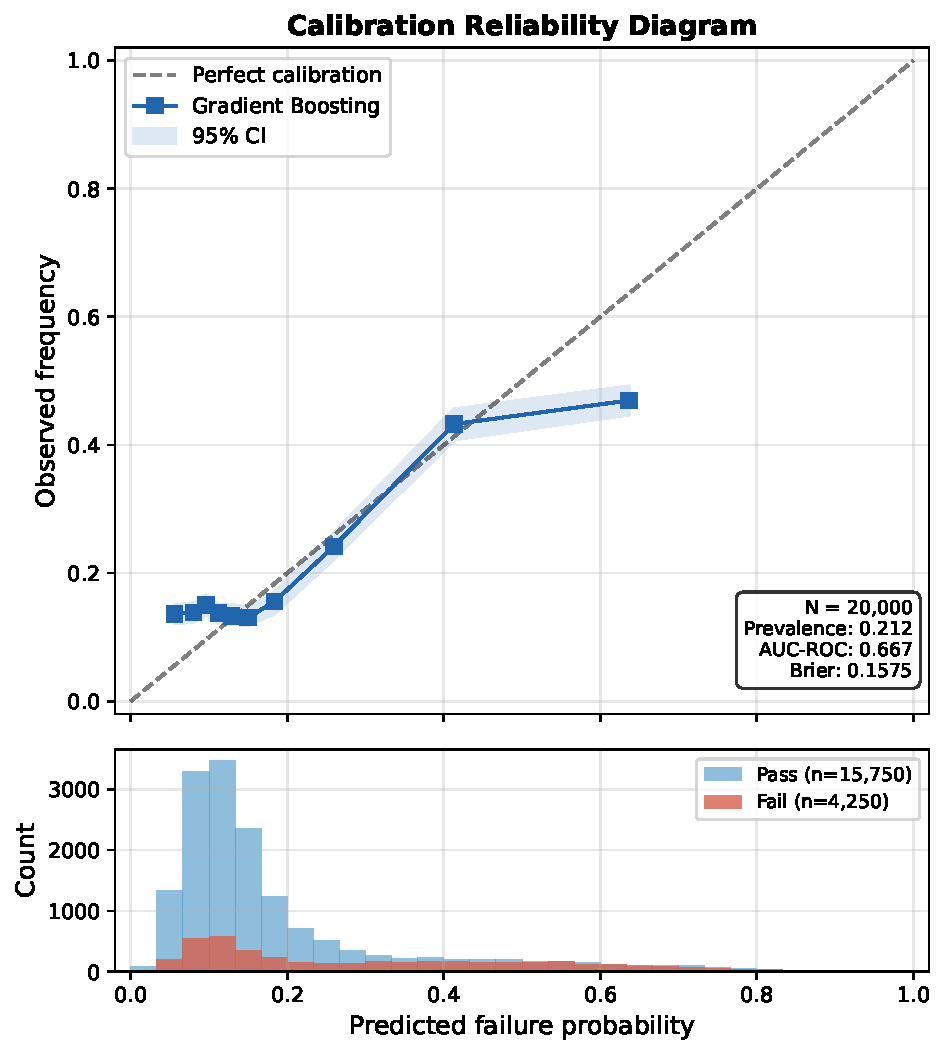
\includegraphics[width=0.85\textwidth]{fig_calibration.pdf}
    \caption{Calibration reliability diagram from cross-validated predictions. Top: predicted vs.\ observed failure probability with 95\% bootstrap confidence band. Bottom: distribution of predicted probabilities by outcome class.}
    \label{fig:calibration}
\end{figure}

For operational deployment, each patient scheduled for the current day is processed through the trained model to obtain $\hat{p}_i = f_\theta(\mathbf{x}_i)$. In our simulation-augmented cohort, predicted probabilities range from 0.01 to 0.96, with a mean of 0.21 reflecting the heterogeneous risk composition of the cohort. This probability parameterizes the patient-specific service time distribution:
\begin{equation}
\Theta_i = \left\{ \left(d_i^0,\, 1 - \hat{p}_i\right),\; \left(d_i^0 + \delta_i,\, \hat{p}_i\right) \right\}
\label{eq:bernoulli_params}
\end{equation}
where $d_i^0$ denotes the nominal procedure duration and $\delta_i$ denotes the time penalty incurred upon failure (repositioning, rescanning, or session termination). This Bernoulli-weighted mixture distribution serves as the stochastic foundation for the scheduling optimization developed in Section~\ref{sec:scheduling_formulation}.


%==============================================================================
% SECTION 2.3: STOCHASTIC SCHEDULING FORMULATION
%==============================================================================

\subsection{Stochastic Multi-Modal Scheduling Formulation}
\label{sec:scheduling_formulation}

We formulate the clinical trial scheduling problem as a stochastic flexible job-shop model with patient-specific service time distributions derived from the predictive component. This section presents the mathematical program, discusses the relationship between scenario-based stochastic programming and the computationally tractable expected-value formulation we implement, and establishes the theoretical foundations for the scheduling optimization.

\subsubsection{Problem Setting and Notation}

Consider a clinical research facility scheduling $n$ patients across $m$ sequential diagnostic modalities on a given operational day. Each patient must complete all modalities in a fixed precedence order dictated by clinical protocol---for example, the UDS clinical interview must precede MRI neuroimaging, which must precede CSF lumbar puncture. Each modality is serviced by a single resource (one interview room, one MRI scanner, one procedure room), creating resource contention that the scheduling model must resolve.

Let $\mathcal{I} = \{1, 2, \ldots, n\}$ denote the set of patients and $\mathcal{J} = \{1, 2, \ldots, m\}$ denote the set of clinical resources (modalities). For each patient $i \in \mathcal{I}$, define the ordered sequence of operations $\mathcal{S}_i = (O_{i,1}, O_{i,2}, \ldots, O_{i,m})$ where $O_{i,s}$ denotes the $s$-th operation for patient $i$, requiring resource $j(s) \in \mathcal{J}$.

\subsubsection{Stochastic Service Time Model}

The distinguishing feature of our formulation is the patient-specific stochastic characterization of service times. For patient $i$ on resource $j$, the service time $D_{ij}$ is a random variable following the Bernoulli-weighted distribution:
\begin{equation}
D_{ij} = 
\begin{cases}
d_{ij}^0 & \text{with probability } (1 - p_{ij}) \\
d_{ij}^0 + \delta_{ij} & \text{with probability } p_{ij}
\end{cases}
\label{eq:service_time_rv}
\end{equation}

where $d_{ij}^0$ denotes the nominal processing time of patient $i$ on resource $j$, $p_{ij}$ denotes the ML-predicted failure probability, and $\delta_{ij}$ denotes the time penalty incurred upon failure (repositioning, rescanning, or session termination).

The failure probabilities $p_{ij}$ derive from the predictive model of Section~\ref{sec:predictive_model}. For the MRI resource, $p_{i,\text{MRI}} = \hat{p}_i$ directly. For other resources, we scale proportionally based on the procedural demands each modality places on patient cooperation: $p_{i,\text{UDS}} = 0.3 \cdot \hat{p}_i$ and $p_{i,\text{CSF}} = 0.8 \cdot \hat{p}_i$. The UDS clinical interview is conducted conversationally and tolerates brief lapses in attention or mild agitation without requiring procedure restart; the interviewer can pause, redirect, and adapt pacing to the patient's state, substantially reducing the probability that cognitive or behavioral impairment precipitates procedural failure. In contrast, CSF collection via lumbar puncture requires the patient to maintain a sustained flexed position for the duration of needle insertion and fluid collection, imposing physical stillness demands comparable to MRI acquisition. The 0.8 scaling factor reflects that while lumbar puncture is shorter than MRI, the consequences of patient movement during needle placement are clinically significant.

We note that these scaling factors represent informed clinical judgment rather than empirically estimated parameters. A dedicated sensitivity analysis varying each factor by $\pm 50\%$ across nine combinations (Section~\ref{sec:value_analysis}, Table~\ref{tab:scaling_sensitivity}) confirms that the main findings---prediction quality dominating optimization sophistication, and LPT achieving near-optimal performance---are robust to the specific scaling values chosen, with LPT overtime probability varying by only 1.57 percentage points across the perturbation grid.

\subsubsection{Decision Variables}

The scheduling model determines:
\begin{align}
x_{ij} &\geq 0 && \text{Start time of patient } i \text{ on resource } j \\
y_{ii'j} &\in \{0, 1\} && \text{1 if patient } i \text{ precedes patient } i' \text{ on resource } j \\
C_{\max} &\geq 0 && \text{Makespan (completion time of last operation)} \\
W_i &\geq 0 && \text{Total waiting time for patient } i \text{ between operations}
\end{align}


To illustrate the operational meaning of the stochastic service time model, consider an MRI scan with nominal duration $d^0 = 45$ minutes, failure penalty $\delta = 30$ minutes, and ML-predicted failure probability $p_i = 0.20$. With probability 0.80, the scan completes successfully in 45 minutes; with probability 0.20, a failure event extends the session to 75 minutes. The risk-adjusted expected duration is $\tilde{d} = 45 + 0.20 \times 30 = 51$ minutes, allocating 6 minutes of buffer proportional to the patient's individualized risk. A low-risk patient with $p_i = 0.05$ would receive only 1.5 minutes of buffer ($\tilde{d} = 46.5$), while a high-risk patient with $p_i = 0.45$ would receive 13.5 minutes ($\tilde{d} = 58.5$). This proportional allocation is the mechanism by which ML-predicted probabilities translate into differentiated scheduling decisions.


\subsubsection{Scenario-Based Stochastic Programming Formulation}

The theoretically complete formulation employs sample average approximation (SAA), generating $K$ scenarios $\omega_1, \ldots, \omega_K$ by sampling from the patient-specific service time distributions \eqref{eq:service_time_rv}. For each scenario $\omega_k$, the realized service time $d_{ij}(\omega_k)$ equals either $d_{ij}^0$ or $d_{ij}^0 + \delta_{ij}$ according to independent Bernoulli draws with success probability $p_{ij}$.

The two-stage stochastic program minimizes expected costs across scenarios:
\begin{equation}
\min_{x, y} \; \frac{1}{K} \sum_{k=1}^{K} \left[ C_{\max}(\omega_k) + \lambda \sum_{i \in \mathcal{I}} W_i(\omega_k) \right]
\label{eq:saa_objective}
\end{equation}
where $\lambda \geq 0$ weights the trade-off between clinic efficiency (makespan) and patient experience (waiting time).

The scenario-dependent constraints for each $\omega_k$ include precedence requirements ensuring operation sequence, disjunctive constraints preventing resource conflicts, and linking constraints defining makespan and waiting times in terms of realized service durations $d_{ij}(\omega_k)$.

\subsubsection{Expected-Value Formulation}

While scenario-based SAA preserves the full distributional information encoded in the ML-predicted probabilities, it introduces significant computational burden: the number of binary sequencing variables scales as $O(n^2 m K)$, rendering large instances intractable for real-time operational deployment. Following the computational tractability arguments established in the stochastic scheduling literature \citep{denton2003sequential, mancilla2012sample}, we implement an expected-value formulation that captures patient-specific risk heterogeneity while maintaining practical solvability.

The expected-value formulation replaces the random service time $D_{ij}$ with its expectation:
\begin{equation}
\tilde{d}_{ij} = \mathbb{E}[D_{ij}] = d_{ij}^0 + p_{ij} \cdot \delta_{ij}
\label{eq:expected_duration}
\end{equation}

This risk-adjusted duration allocates buffer time proportionally to predicted failure probability: a patient with $p_{ij} = 0.30$ and penalty $\delta_{ij} = 30$ minutes receives $0.30 \times 30 = 9$ minutes of expected buffer beyond the nominal duration, while a low-risk patient with $p_{ij} = 0.02$ receives only 0.6 minutes.

The deterministic equivalent formulation becomes:

\textbf{Objective Function:}
\begin{equation}
\min \; Z = C_{\max} + \lambda \sum_{i \in \mathcal{I}} W_i
\label{eq:objective}
\end{equation}

\textbf{Precedence Constraints:} Each patient must complete their current operation before beginning the next in sequence. For patient $i$ and consecutive operations on resources $j$ (current) and $k$ (next):
\begin{equation}
x_{ik} \geq x_{ij} + \tilde{d}_{ij} \quad \forall i \in \mathcal{I}, \; \forall (j, k) \in \mathcal{S}_i
\label{eq:precedence}
\end{equation}

\textbf{Patient Waiting Time Definition:} The waiting time for patient $i$ accumulates across transitions between consecutive operations:
\begin{equation}
W_i = \sum_{(j,k) \in \mathcal{S}_i} \left( x_{ik} - x_{ij} - \tilde{d}_{ij} \right) \quad \forall i \in \mathcal{I}
\label{eq:wait_time}
\end{equation}

\textbf{Disjunctive Resource Constraints:} Each resource can process only one patient at a time. For any pair of patients $i, i' \in \mathcal{I}$ with $i \neq i'$ requiring resource $j$, exactly one must precede the other:
\begin{align}
x_{i'j} &\geq x_{ij} + \tilde{d}_{ij} - M(1 - y_{ii'j}) \label{eq:disjunctive1} \\
x_{ij} &\geq x_{i'j} + \tilde{d}_{i'j} - M \cdot y_{ii'j} \label{eq:disjunctive2}
\end{align}
where $M$ is a sufficiently large constant. When $y_{ii'j} = 1$, constraint \eqref{eq:disjunctive1} enforces that patient $i$ precedes patient $i'$ on resource $j$, while constraint \eqref{eq:disjunctive2} becomes redundant. The converse holds when $y_{ii'j} = 0$.

\textbf{Makespan Definition:}
\begin{equation}
C_{\max} \geq x_{ij} + \tilde{d}_{ij} \quad \forall i \in \mathcal{I}, \; \forall j \in \mathcal{J}
\label{eq:makespan}
\end{equation}

\textbf{Variable Domains:}
\begin{align}
x_{ij} &\geq 0 && \forall i \in \mathcal{I}, \; \forall j \in \mathcal{J} \\
y_{ii'j} &\in \{0, 1\} && \forall i \neq i' \in \mathcal{I}, \; \forall j \in \mathcal{J} \\
C_{\max}, W_i &\geq 0 && \forall i \in \mathcal{I}
\end{align}

\subsubsection{Theoretical Justification for Expected-Value Approximation}

The expected-value formulation \eqref{eq:expected_duration} constitutes a first-order approximation to the scenario-based stochastic program \eqref{eq:saa_objective}. Several theoretical and practical considerations justify this approximation for our application context.

First, \citet{denton2003sequential} established that for convex piecewise-linear cost structures---which characterize waiting time and overtime costs---the expected-value solution provides a bound on the stochastic optimum. While our job-shop formulation with integer sequencing variables is not convex, the insight that expected-value solutions perform well when variance is moderate relative to means remains applicable.

Second, the Bernoulli service time distribution \eqref{eq:service_time_rv} has coefficient of variation:
\begin{equation}
\text{CV}_{ij} = \frac{\sqrt{p_{ij}(1-p_{ij})} \cdot \delta_{ij}}{d_{ij}^0 + p_{ij} \cdot \delta_{ij}}
\end{equation}
For typical parameter values ($d_{ij}^0 = 45$ min, $\delta_{ij} = 30$ min, $p_{ij} \leq 0.30$), this coefficient of variation remains below 0.25, indicating that the expected-value summary captures most of the distributional information relevant to sequencing decisions.

Third, the sequencing decisions encoded in the binary variables $y_{ii'j}$ are robust to moderate perturbations in duration estimates. The optimal sequence depends on the relative ordering of risk-adjusted durations $\tilde{d}_{ij}$ across patients, which is preserved under expected-value computation. Scenario-based approaches would yield different makespan realizations across scenarios but similar optimal sequences, suggesting that the expected-value formulation captures the decision-relevant structure.

Fourth, operational deployment requires solution times compatible with daily scheduling cycles. The expected-value formulation with $n = 10$ patients and $m = 3$ resources yields approximately 100 constraints and 50 binary variables, solvable to optimality within 60 seconds using commercial mixed-integer programming solvers. Scenario-based SAA with $K = 100$ scenarios would inflate the problem by two orders of magnitude, exceeding practical time limits for real-time decision support.

\subsubsection{Symmetry-Breaking and Computational Enhancements}

The disjunctive constraints \eqref{eq:disjunctive1}--\eqref{eq:disjunctive2} introduce substantial symmetry: any permutation of patients with identical risk-adjusted durations yields equivalent solutions. To accelerate convergence, we impose symmetry-breaking constraints that fix the sequencing of patients whose risk ordering is unambiguous:
\begin{equation}
y_{ii'j} = 1 \quad \text{if } \tilde{d}_{ij} > \tilde{d}_{i'j} + \epsilon
\label{eq:symmetry_breaking}
\end{equation}
for a small tolerance $\epsilon > 0$. This constraint encodes the intuition that higher-risk patients (with longer expected durations) should be scheduled earlier, providing buffer time for potential delays without cascading effects on subsequent patients.

Additionally, we construct an initial feasible solution using a longest-processing-time-first (LPT) heuristic, warm-starting the branch-and-bound search. The LPT solution provides an upper bound that enables aggressive pruning of the search tree.

\subsubsection{Managerial Interpretation}

The formulation embeds several operationally significant features. The risk-adjusted durations $\tilde{d}_{ij}$ translate ML-predicted failure probabilities into tangible schedule modifications: a patient identified as high-risk receives proportionally more allocated time, reducing the probability of cascading delays. The waiting time penalty $\lambda$ enables clinic managers to balance institutional efficiency against patient experience---higher $\lambda$ values produce schedules with minimal inter-procedure gaps at the cost of potentially extended makespans. The precedence constraints encode clinical protocol requirements, ensuring that data collection sequences mandated by trial design are respected.

The symmetry-breaking constraints \eqref{eq:symmetry_breaking} operationalize a risk-management heuristic: scheduling high-risk patients early in the day provides recovery time if failures occur, while low-risk patients scheduled later face minimal delay probability. This sequencing logic emerges naturally from the optimization rather than requiring manual specification, demonstrating how the prescriptive framework translates predictive information into actionable scheduling decisions.

%==============================================================================
% SECTION 3: COMPUTATIONAL EXPERIMENTS
%==============================================================================


\section{Experiments}
\label{sec:experiments}

This section evaluates the prescriptive analytics framework through computational experiments designed to decompose scheduling performance into its constituent sources of value. By systematically varying both the prediction method and the optimization approach, we isolate the relative contributions of prediction quality, feature richness, and optimization sophistication. Seven scheduling methods are compared, ranging from no prediction (deterministic) through simple stratification (age-based rules) to full ML prediction using cognitive and behavioral biomarkers, paired with both heuristic sequencing and mixed-integer programming optimization.

\subsection{Experimental Setup}
\label{sec:experimental_setup}

We generate patient cohorts using simulation-augmented clinical profiles calibrated to published distributions for Alzheimer's disease patient populations. Each experimental instance comprises $n = 10$ patients sampled to reflect realistic cohort heterogeneity, with approximately 25\% classified as high-risk ($p_i > 0.25$) based on their clinical profiles. Patient features (age, MoCA, CDR, NPI-Q behavioral symptoms) are drawn from clinically realistic distributions, and failure probabilities ranging from 0.03 to 0.55 are determined by the nonlinear relationship between these features and procedural risk documented by \citet{porembka2025disparities}. This simulation-augmented approach is necessary because well-managed research settings, with their extensive pre-screening protocols, yield near-zero observed failure rates that do not reflect the 10--30\% rates observed in routine clinical practice with cognitively impaired populations. \rev{Section~\ref{sec:real_data_arm} complements these simulation-augmented instances with a second evaluation arm in which cohorts are sampled from real NACC participant records under the same experimental protocol.}

Table~\ref{tab:resource_params} summarizes the clinical resource parameters. The UDS clinical interview requires 60 minutes base duration with a 15-minute failure penalty. MRI neuroimaging requires 45 minutes base duration with a 30-minute penalty, serving as the primary bottleneck resource. CSF lumbar puncture requires 30 minutes with a 20-minute penalty. Risk scaling factors translate the MRI-derived failure probability $\hat{p}_i$ into resource-specific values $p_{i,j}$ that reflect each modality's tolerance for patient movement and behavioral disruption. We use 1.0 for MRI by construction ($p_{i,\text{MRI}} = \hat{p}_i$), 0.3 for UDS, and 0.8 for CSF. The lower factor for UDS reflects that the interview is conversational: an interviewer can pause, redirect, and adapt pacing to the patient's state, so cognitive lapses or mild agitation rarely precipitate procedural restart. The higher factor for CSF reflects that lumbar puncture, although shorter than MRI, requires sustained flexed positioning during needle placement, making patient movement clinically consequential. These factors represent informed clinical judgment rather than empirically estimated parameters; their full mechanistic justification appears in Section~\ref{sec:scheduling_formulation}, and a dedicated sensitivity analysis (Section~\ref{sec:value_analysis}, Table~\ref{tab:scaling_sensitivity}) confirms robustness: perturbing each factor by $\pm 50\%$ across nine combinations preserves the qualitative findings, with LPT remaining within 0.47 percentage points of Stochastic-MILP and both continuing to dominate Age-Stratified scheduling.

\begin{table}[htbp]
\centering
\caption{Clinical resource parameters}
\label{tab:resource_params}
\begin{tabular}{@{}lccc@{}}
\toprule
\textbf{Resource} & \textbf{Base Duration} $d^0$ & \textbf{Failure Penalty} $\delta$ & \textbf{Risk Scale} \\
\midrule
UDS Clinical Interview & 60 min & 15 min & 0.3 \\
MRI Neuroimaging & 45 min & 30 min & 1.0 \\
CSF Lumbar Puncture & 30 min & 20 min & 0.8 \\
\bottomrule
\end{tabular}
\end{table}

All experiments were conducted using Python 3.11 with the PuLP optimization library interfacing the CBC mixed-integer programming solver. Schedule quality is assessed through Monte Carlo simulation: for each schedule, we simulate 100 stochastic realizations where actual service times are drawn from the Bernoulli distributions parameterized by true failure probabilities. This evaluation captures the distinction between planned performance and realized performance under operational variability. We report expected makespan (mean across simulations) and overtime probability (fraction of simulations exceeding planned makespan by more than 5\%).

\subsection{Baseline Methods}
\label{sec:baselines}

We compare seven scheduling approaches that differ in their use of predictive information. The Stochastic-MILP method represents our proposed framework, using ML-predicted failure probabilities to compute risk-adjusted expected durations and optimizing via mixed-integer programming. LPT (Longest Processing Time) orders patients by total risk-adjusted duration with highest-risk patients first, representing a simple heuristic that exploits ML predictions without optimization. SPT (Shortest Processing Time) applies the reverse ordering, scheduling lowest-risk patients first. FCFS (First-Come-First-Served) maintains arrival order with risk-adjusted durations, representing typical clinical practice with ML predictions but no intelligent sequencing. Random ordering provides a lower bound, averaged over 10 samples.

Two baselines specifically test the value of ML predictions. The Deterministic baseline uses nominal durations only, ignoring failure risk entirely and thus requiring no predictive model. The Age-Stratified baseline applies rule-based buffers without machine learning: 5\% of the failure penalty for ages 65--74, 15\% for ages 75--84, and 25\% for ages 85+. The bracket structure follows the standard geriatric stratification used widely in age-related epidemiological research and adopted in the motion-artifact analysis of \citet{porembka2025disparities}; the buffer percentages are deliberately set proportional to the documented odds-ratio range for age-related motion-artifact risk in that study (approximately 1.5--3.3 across age strata), translated into roughly increasing buffer allocations that embody a credible---rather than minimal or extreme---form of demographic-based clinical intuition. We emphasize that the specific values are illustrative of this class of heuristic rather than empirically optimized; what the comparison tests is whether \emph{any} simple demographic rule of this form can match risk-aware sequencing informed by cognitive and behavioral covariates. As the results in Section~\ref{sec:results} show, it cannot---a pattern consistent across the parameter range explored in the scaling-factor sensitivity analysis of Section~\ref{sec:value_analysis}.


\subsection{Results}
\label{sec:results}

Table~\ref{tab:baseline_results} presents results from 100 independent replications, each with a randomly sampled 10-patient cohort evaluated through 100 Monte Carlo simulations.

\begin{table}[htbp]
\centering
\caption{Baseline comparison results (100 replications, 10 patients each, 100 simulations per schedule). Values show mean $\pm$ 95\% confidence interval.}
\label{tab:baseline_results}
\begin{tabular}{@{}lcc@{}}
\toprule
\textbf{Method} & \textbf{Expected Makespan (min)} & \textbf{Overtime Probability} \\
\midrule
LPT & 689.0 $\pm$ 0.4 & 3.0\% $\pm$ 0.4\% \\
Stochastic-MILP & 689.1 $\pm$ 0.4 & 3.1\% $\pm$ 0.4\% \\
Deterministic & 689.0 $\pm$ 0.4 & 9.4\% $\pm$ 0.8\% \\
Random & 695.4 $\pm$ 0.7 & 6.2\% $\pm$ 0.5\% \\
FCFS & 698.1 $\pm$ 1.2 & 7.0\% $\pm$ 0.7\% \\
SPT & 715.0 $\pm$ 0.7 & 9.8\% $\pm$ 0.7\% \\
Age-Stratified & 692.4 $\pm$ 0.6 & 12.2\% $\pm$ 1.0\% \\
\bottomrule
\end{tabular}
\end{table}

The results reveal a striking pattern: the primary determinant of scheduling performance is whether ML predictions are used effectively, not whether optimization is employed. The LPT heuristic and Stochastic-MILP achieve statistically indistinguishable performance (3.0\% vs 3.1\% overtime, $p > 0.05$), both substantially outperforming all other methods. This convergence occurs because the symmetry-breaking constraints in our MILP formulation encode risk-first sequencing logic, and for the instances tested, this sequencing dominates the objective. The practical implication is significant: practitioners can implement a simple sorting rule---schedule patients in decreasing order of predicted risk---and achieve near-optimal performance without requiring optimization software.

However, this simplicity depends critically on having accurate patient-specific predictions. The Age-Stratified baseline, which uses only patient age to allocate scheduling buffer, achieves 12.2\% overtime probability---four times higher than methods using full ML predictions. The 9.2 percentage point improvement from Age-Stratified to LPT quantifies the value of ML prediction over intuitive heuristics, arising because age alone is a weak proxy for the failure risk that cognitive and behavioral features capture (Section~\ref{sec:value_analysis}).

The Deterministic baseline presents an instructive case. Its expected makespan matches LPT and Stochastic-MILP (689 minutes), yet its overtime probability is three times higher (9.4\% vs 3.0\%). This occurs because Deterministic schedules ignore variability: they appear efficient on paper but provide no buffer for failure events. When failures occur, they cascade through the schedule.

\subsubsection{Computational Efficiency}

Table~\ref{tab:computation_times} reports wall-clock computation times across 50 replications, quantifying the practical cost of optimization sophistication.

\begin{table}[H]
\centering
\caption{Computation times for scheduling methods ($n = 10$ patients, 50 replications).}
\label{tab:computation_times}
\begin{tabular}{lcccc}
\toprule
Method & Mean (s) & Std (s) & Min (s) & Max (s) \\
\midrule
FCFS & 0.0009 & 0.0000 & 0.0009 & 0.0010 \\
SPT & 0.0006 & 0.0000 & 0.0006 & 0.0007 \\
LPT & 0.0006 & 0.0000 & 0.0006 & 0.0008 \\
Deterministic & 0.0006 & 0.0000 & 0.0006 & 0.0008 \\
Age-Stratified & 0.0006 & 0.0000 & 0.0006 & 0.0009 \\
Random & 0.0059 & 0.0001 & 0.0057 & 0.0063 \\
Stochastic-MILP & 20.7819 & 19.3779 & 0.1277 & 60.1351 \\
\bottomrule
\end{tabular}
\end{table}

The computational disparity is striking. All heuristic methods solve in under one millisecond, while the Stochastic-MILP averages 20.8 seconds with a maximum of 60.1 seconds (reaching the solver timeout). The high variance in MILP solve times (standard deviation of 19.4 seconds) reflects the branch-and-bound search tree's sensitivity to patient-specific parameter values. Given the statistically indistinguishable scheduling quality between LPT and Stochastic-MILP (Table~\ref{tab:baseline_results}), this $35{,}000\times$ computational overhead yields no measurable operational benefit for the problem instances tested. For real-time deployment where schedules must be computed daily, the sub-millisecond LPT solution is operationally preferable.

\subsection{Scalability Analysis}
\label{sec:scalability}

The baseline comparison (Table~\ref{tab:baseline_results}) established LPT-MILP equivalence for $n = 10$ patients. A natural question is whether this equivalence holds at realistic clinic volumes, where daily patient throughput may reach 20--50 individuals. Table~\ref{tab:scalability} reports results from scaling experiments with $n \in \{10, 20, 30, 50\}$ patients, using 10 replications per size with solver timeout set to $\max(60, 6n)$ seconds.

\begin{table}[H]
\centering
\caption{Scalability comparison: Stochastic-MILP vs.\ LPT across problem sizes (10 replications per size).}
\label{tab:scalability}
\begin{tabular}{@{}rrrccccr@{}}
\toprule
$n$ & Variables & Constraints & MILP Time (s) & LPT Time & Optimal & MILP Makespan & LPT Makespan \\
\midrule
10 & 176 & 320 & 17.1 $\pm$ 17.3 & 2.1 ms & 9/10 & 687.1 & 687.1 \\
20 & 651 & 1{,}240 & 120.2 $\pm$ 0.0 & 2.1 ms & 0/10 & 1{,}297.0 & 1{,}297.0 \\
30 & 1{,}426 & 2{,}760 & 180.2 $\pm$ 0.0 & 2.2 ms & 0/10 & 1{,}913.1 & 1{,}905.7 \\
50 & --- & --- & --- & 2.3 ms & --- & --- & 3{,}124.8 \\
\bottomrule
\end{tabular}
\end{table}

The scalability results reveal three patterns that substantially strengthen the practical case for LPT. First, the MILP formulation becomes computationally intractable at $n \geq 20$: every instance reaches the solver timeout, and the problem grows quadratically in both decision variables (from 176 to 1{,}426) and constraints (from 320 to 2{,}760). At $n = 50$, the experiment did not produce results within the allocated time. LPT, by contrast, solves in approximately 2~milliseconds regardless of instance size, maintaining a constant-time profile that is operationally suitable for any realistic clinic volume.

Second, the LPT-MILP equivalence that held at $n = 10$ persists at $n = 20$, where the timed-out MILP solutions match LPT makespan exactly (1{,}297.0 minutes). This occurs because the branch-and-bound solver discovers the risk-first ordering as a feasible solution early in its search but cannot prove optimality within the time limit. However, at $n = 30$, a divergence emerges---and it favors LPT. The MILP's mean makespan (1{,}913.1 minutes) exceeds LPT (1{,}905.7 minutes) by 0.39\%, with individual replications showing gaps as large as 27 minutes. This inversion occurs because the solver, unable to explore sufficient nodes within the timeout, sometimes terminates with an inferior feasible solution that the simple LPT heuristic avoids entirely.

Third, LPT overtime probability decreases monotonically with cohort size: from 2.8\% at $n = 10$ to 0.2\% at $n = 20$ and 0.0\% at $n \geq 30$. This reflects the law of large numbers---as the number of patients increases, the realized proportion of failures converges to its expectation, reducing tail risk. The practical implication is that risk-first sequencing becomes \textit{more} effective, not less, at the larger cohort sizes characteristic of real clinical operations.

These findings confirm that LPT is not merely a computationally convenient approximation but the operationally preferred method for realistic clinic sizes. The MILP formulation retains value as a theoretical benchmark for certifying heuristic quality at small scale, but it cannot serve as a practical scheduling tool beyond $n = 20$ patients without substantially more powerful solver infrastructure or problem-specific decomposition methods.


\subsection{Value Decomposition}
\label{sec:value_analysis}

Table~\ref{tab:value_analysis} decomposes the performance improvement into components attributable to prediction quality versus optimization sophistication. The following decomposition quantifies the \textit{structural} contributions of prediction quality and optimization sophistication under the calibrated simulation parameters. While the specific magnitudes would vary with empirical failure rates and feature distributions, the qualitative ordering---prediction dominating optimization---is robust across the parameter ranges tested in the sensitivity analyses reported later in this subsection.

\begin{table}[htbp]
\centering
\caption{Value decomposition: contributions of ML prediction and optimization}
\label{tab:value_analysis}
\begin{tabular}{@{}lcc@{}}
\toprule
\textbf{Comparison} & \textbf{Overtime Reduction} & \textbf{Interpretation} \\
\midrule
LPT vs.\ Age-Stratified & 9.2 pp & Value of ML prediction \\
LPT vs.\ Deterministic & 6.4 pp & Value of risk-adjustment \\
Stochastic-MILP vs.\ LPT & 0.1 pp & Value of optimization \\
\bottomrule
\end{tabular}
\end{table}

The decomposition is clear: nearly all performance improvement derives from ML prediction quality, not optimization sophistication. The transition from Age-Stratified to LPT---both using heuristic sequencing but differing in prediction source---yields 9.2 percentage points of overtime reduction. The transition from LPT to Stochastic-MILP---same predictions but adding optimization---yields only 0.1 percentage points, statistically indistinguishable from zero.

To further isolate the source of predictive value, we conducted an additional experiment comparing four prediction approaches: Full ML using the complete feature set, Age-Only ML using only age-derived features, Age-Stratified using rule-based buffers, and No Prediction using deterministic durations. Table~\ref{tab:ml_value} presents results from 50 independent replications.

\begin{table}[H]
\centering
\caption{Value of ML components (50 replications, 100 simulations each). }
\label{tab:ml_value}
\begin{tabular}{@{}lcc@{}}
\toprule
\textbf{Prediction Approach} & \textbf{Overtime Probability} & \textbf{vs.\ Full ML} \\
\midrule
Full ML & 3.1\% $\pm$ 0.6\% & --- \\
No Prediction & 8.7\% $\pm$ 1.1\% & +5.6 pp \\
Age-Stratified & 11.7\% $\pm$ 1.4\% & +8.5 pp \\
Age-Only ML & 12.0\% $\pm$ 1.6\% & +8.9 pp \\
\bottomrule
\end{tabular}
\end{table}

The results reveal a striking finding: Age-Only ML performs no better than Age-Stratified rules (12.0\% vs 11.7\% overtime, $p > 0.05$). Applying gradient boosting to age features alone provides no advantage over simple stratification. This demonstrates that the value of machine learning derives not from model sophistication but from incorporating cognitive and behavioral biomarkers that age-based approaches cannot capture. The 8.9 percentage point improvement from Age-Only to Full ML quantifies the predictive contribution of MoCA scores, CDR staging, and NPI-Q behavioral symptoms.

An unexpected finding is that No Prediction outperforms both age-based approaches (8.7\% vs 12\% overtime). This occurs because age-based methods actively misallocate scheduling buffers: they assign insufficient slack to cognitively impaired younger patients while over-buffering healthy older patients. The No Prediction baseline, by treating all patients identically, avoids this systematic misallocation---though it still underperforms Full ML by 5.6 percentage points.

The magnitude of the gap between Age-Only and Full ML warrants explanation. As the feature importance analysis in Section~\ref{sec:predictive_model} established, approximately 80\% of predictive signal resides in non-age features---cognitive assessments, dementia staging, and behavioral symptoms. Consider two 78-year-old patients: one with MoCA score 27, CDR 0, and no behavioral symptoms; another with MoCA score 18, CDR 2, and documented agitation. Their true failure probabilities might be 0.08 and 0.45 respectively, yet age-based methods assign identical scheduling buffers. The Full ML model captures these clinically meaningful distinctions, producing individualized risk estimates that enable effective differentiation in scheduling priority.

To assess practical deployment considerations, we tested robustness to prediction error by adding Gaussian noise ($\sigma = 0.05$ to $0.20$) to the ML-predicted probabilities before scheduling, then evaluating against true failure rates. The results indicate graceful degradation: overtime probability increases from 3.1\% with perfect predictions to 5.7\% with 5\% noise and plateaus at approximately 7.6\% for noise levels of 10\% or higher. Notably, even with 20\% prediction error, the ML-based approach (7.6\% overtime) still outperforms Age-Stratified scheduling (11.7\% overtime). This robustness suggests that the framework retains practical value even when deployed with imperfect predictions, as would be expected in real-world clinical settings where model calibration may drift over time.

The benefit of risk-adjusted scheduling also depends on cohort composition. We varied the proportion of high-risk patients from 0\% to 50\% and compared the ML-based approach against deterministic scheduling. The improvement grows substantially with cohort risk: at 0\% high-risk patients, the overtime reduction is 1.2 percentage points (5.8\% to 4.6\%); at 50\% high-risk, it reaches 13.6 percentage points (19.4\% to 5.8\%). While deterministic scheduling degrades sharply as cohort risk increases, the ML-based approach remains stable at 4--6\% overtime across all compositions. This pattern suggests that facilities serving high-risk populations---such as specialized dementia clinics or late-stage Alzheimer's trials---would realize the greatest operational benefit from implementing risk-adjusted scheduling. From a calibration-validity perspective, the 0--50\% sweep brackets the published 10--30\% range used to set the nominal cohort failure rate of 21.2\%, and the qualitative dominance of risk-first scheduling holds throughout this interval. The framework therefore does not depend on the specific midpoint value chosen.

Finally, we examine sensitivity to the resource-specific risk scaling factors that translate the MRI-derived failure probability $\hat{p}_i$ into UDS and CSF failure probabilities ($p_{i,\text{UDS}} = 0.3 \cdot \hat{p}_i$ and $p_{i,\text{CSF}} = 0.8 \cdot \hat{p}_i$ at baseline). We perturb each factor by $\pm 50\%$, generating nine combinations on the grid $\text{UDS} \in \{0.15, 0.30, 0.45\}$ and $\text{CSF} \in \{0.40, 0.80, 1.20\}$, and re-run the comparison of LPT, Stochastic-MILP, Deterministic, and Age-Stratified scheduling at each combination using 30 cohorts and 100 Monte Carlo simulations per schedule. Table~\ref{tab:scaling_sensitivity} reports overtime probability per method per combination.

The qualitative findings of Section~\ref{sec:results} are preserved across all nine combinations, and in two respects the sensitivity analysis strengthens them. First, LPT and Stochastic-MILP remain statistically indistinguishable: the maximum absolute gap between them is 0.47 percentage points, with LPT slightly outperforming MILP in every combination---the same inversion documented in the scalability analysis (Section~\ref{sec:scalability}), now visible at $n=10$ as well. Second, the dominance of risk-aware sequencing over alternatives \emph{widens} as scaling factors increase: LPT overtime varies within a narrow band of 2.40--3.97\% across the nine combinations (range 1.57 percentage points), whereas Deterministic varies from 4.10\% to 15.33\% (range 11.23 percentage points) and Age-Stratified varies from 6.13\% to 17.93\% (range 11.80 percentage points). Risk-first sequencing therefore not only achieves the best mean performance but is also the most robust to miscalibration of the resource-specific scaling factors, while baselines that do not exploit patient-specific risk predictions degrade as the failure-probability budget across resources grows.

\begin{table}[htbp]
\centering
\caption{Sensitivity of scheduling performance to resource-specific risk scaling factors. Each cell reports overtime probability (\%) averaged over 30 cohort replications $\times$ 100 Monte Carlo simulations per schedule. The baseline combination is $(\text{UDS}, \text{CSF}) = (0.30, 0.80)$. The MRI scaling factor is fixed at 1.0 throughout. "Range" is the difference between the maximum and minimum overtime probability for each method across the nine combinations.}
\label{tab:scaling_sensitivity}
\begin{tabular}{@{}cc cccc@{}}
\toprule
\textbf{UDS} & \textbf{CSF} & \textbf{LPT} & \textbf{Stoch-MILP} & \textbf{Determ.} & \textbf{Age-Strat.} \\
\midrule
0.15 & 0.40 & 3.43 & 3.70 & 4.10  & 6.13 \\
0.15 & 0.80 & 3.67 & 3.87 & 5.17  & 7.03 \\
0.15 & 1.20 & 3.97 & 4.27 & 6.20  & 8.23 \\
0.30 & 0.40 & 2.40 & 2.50 & 7.27  & 10.37 \\
0.30 & 0.80 & 3.03 & 3.23 & 8.70  & 11.37 \\
0.30 & 1.20 & 3.27 & 3.37 & 10.27 & 12.70 \\
0.45 & 0.40 & 3.17 & 3.43 & 12.20 & 14.90 \\
0.45 & 0.80 & 3.57 & 3.90 & 13.73 & 16.30 \\
0.45 & 1.20 & 3.80 & 4.27 & 15.33 & 17.93 \\
\midrule
\multicolumn{2}{l}{\textbf{Range}}     & 1.57 & 1.77 & 11.23 & 11.80 \\
\bottomrule
\end{tabular}
\end{table}




%==============================================================================
% NEW SUBSECTION (real-data extension): REAL-COHORT EVALUATION ARM
%==============================================================================
{\color{red}
\subsection{Real-Data Evaluation Arm: Cohorts Sampled from NACC Participant Records}
\label{sec:real_data_arm}

The experiments reported so far evaluate the framework on simulation-augmented cohorts whose covariates are drawn from calibrated marginal distributions. A natural concern is whether the findings depend on that generator: real clinical populations exhibit joint covariate structure---correlations among age, cognition, dementia staging, and behavioral symptoms, and heavy tails within strata---that independent calibrated draws cannot fully capture. To address this concern we add a second evaluation arm in which every experiment is re-run with patient cohorts sampled from real participant records in the NACC Uniform Data Set (June 2026 data freeze), while the simulation-augmented experiments reported above remain unchanged. The two arms are reported side by side: convergent results indicate robustness to the covariate-generating process, whereas divergence would delineate boundary conditions.

\subsubsection{Design}

We pool UDS visits collected under protocol versions 3 and 4 (harmonized through a variable crosswalk; the cognitive, behavioral, and staging variables used by the framework are name-identical across versions) and retain, for each participant, the most recent visit with non-missing age, MoCA total score, and CDR global score. This yields a sampling pool of 30{,}167 participants across NACC's contributing Alzheimer's Disease Research Centers, of whom 18.8\% meet the high-risk staging criterion (CDR global $\geq 1$)---a naturally leaner case mix than the 25\% high-risk fraction of the synthetic generator. Each experimental replication draws a fresh cohort of the required size from this pool, with a distinct random seed per replication. Cohorts preserve the pool's natural case mix, except in the cohort-composition experiment, where sampling is stratified on CDR global $\geq 1$ to control the high-risk fraction exactly as in the synthetic design.

Because NACC's pre-screened research setting cannot supply operational failure outcomes (Section~\ref{sec:limitations}), the failure-probability mapping is kept identical to the synthetic arm: the same published-rate-calibrated functional form maps each participant's real covariates (age, MoCA, CDR global) to a failure probability, with the pool mean recalibrated to the 21.2\% published midpoint. The real arm therefore isolates exactly one design factor---where the covariates come from---so that any difference between arms is attributable to real covariate heterogeneity. All other protocol elements (replication counts, 100 Monte Carlo simulations per schedule, solver time limits, random seeds) match the corresponding simulation-augmented experiments.

\subsubsection{Results: The Central Finding Replicates and Strengthens}

Table~\ref{tab:real_baseline} reports the baseline comparison on real cohorts (100 replications, 10 patients, 100 simulations per schedule) side by side with Table~\ref{tab:baseline_results}.

\begin{table}[H]
\centering
\color{red}
\caption{Baseline comparison on real NACC cohorts, side by side with the simulation-augmented results of Table~\ref{tab:baseline_results}. Values show mean $\pm$ 95\% confidence interval.}
\label{tab:real_baseline}
\begin{tabular}{@{}lcccc@{}}
\toprule
& \multicolumn{2}{c}{\textbf{Simulation-augmented}} & \multicolumn{2}{c}{\textbf{Real NACC cohorts}} \\
\cmidrule(lr){2-3} \cmidrule(lr){4-5}
\textbf{Method} & \textbf{Makespan (min)} & \textbf{Overtime} & \textbf{Makespan (min)} & \textbf{Overtime} \\
\midrule
LPT & 689.0 $\pm$ 0.4 & 3.0\% $\pm$ 0.4\% & 691.0 $\pm$ 0.7 & 4.4\% $\pm$ 0.5\% \\
Stochastic-MILP & 689.1 $\pm$ 0.4 & 3.1\% $\pm$ 0.4\% & 691.1 $\pm$ 0.7 & 4.4\% $\pm$ 0.5\% \\
Deterministic & 689.0 $\pm$ 0.4 & 9.4\% $\pm$ 0.8\% & 691.0 $\pm$ 0.7 & 12.7\% $\pm$ 1.2\% \\
Random & 695.4 $\pm$ 0.7 & 6.2\% $\pm$ 0.5\% & 697.5 $\pm$ 1.3 & 8.1\% $\pm$ 0.8\% \\
FCFS & 698.1 $\pm$ 1.2 & 7.0\% $\pm$ 0.7\% & 697.4 $\pm$ 1.5 & 7.6\% $\pm$ 0.9\% \\
SPT & 715.0 $\pm$ 0.7 & 9.8\% $\pm$ 0.7\% & 712.9 $\pm$ 1.9 & 11.1\% $\pm$ 1.1\% \\
Age-Stratified & 692.4 $\pm$ 0.6 & 12.2\% $\pm$ 1.0\% & 698.1 $\pm$ 1.7 & 21.9\% $\pm$ 2.8\% \\
\bottomrule
\end{tabular}
\end{table}

Three observations stand out. First, the LPT--MILP equivalence is, if anything, sharper on real cohorts: the two methods coincide to one decimal place in both expected makespan and overtime probability, while the MILP still averages 17.3 seconds per instance (maximum 60.1 s, the solver time limit) against sub-millisecond LPT. The value decomposition of Table~\ref{tab:value_analysis}, re-computed on real cohorts, attributes 17.5 percentage points of overtime reduction to ML prediction (LPT vs.\ Age-Stratified), 8.3 points to risk adjustment (LPT vs.\ Deterministic), and 0.0 points to optimization (Stochastic-MILP vs.\ LPT).

Second, the penalty for age-based scheduling nearly doubles: Age-Stratified overtime rises from 12.2\% on simulation-augmented cohorts to 21.9\% on real cohorts. The mechanism is the one identified in Section~\ref{sec:value_analysis}---systematic misallocation from an inadequate proxy---amplified because the real joint distribution decouples age from cognition more strongly than the synthetic generator assumed: cognitively intact older participants and impaired younger participants, both common in the NACC pool, are precisely the cases that age-based buffers mishandle. The ML-value experiment repeated on real cohorts (50 replications) confirms this: Full ML 4.3\% $\pm$ 0.6\%, No Prediction 12.6\% $\pm$ 1.6\%, Age-Only ML 21.0\% $\pm$ 3.3\%, Age-Stratified 21.9\% $\pm$ 4.0\%. Age-restricted machine learning again fails to improve on age-bracket rules, No Prediction again outperforms both age-based methods (now by 8--9 rather than approximately 3 percentage points), and the Full-ML advantage over Age-Only ML widens from 8.9 to 16.7 percentage points.

Third, overtime levels shift upward by roughly one to ten percentage points across all methods, consistent with heavier-tailed real covariate heterogeneity; the methods' ordering and pairwise gaps are preserved throughout. The simulation-augmented experiments therefore appear, if anything, to \textit{understate} the operational value of full-feature prediction.

\subsubsection{Replication of the Remaining Experiments}

Table~\ref{tab:real_replication} summarizes the real-cohort replication of the scalability, prediction-error, cohort-composition, and scaling-factor-sensitivity experiments, run under the same designs as Sections~\ref{sec:scalability} and~\ref{sec:value_analysis}.

\begin{table}[H]
\centering
\color{red}
\caption{Replication of the remaining experiments on real NACC cohorts (same designs as Sections~\ref{sec:scalability} and~\ref{sec:value_analysis}).}
\label{tab:real_replication}
\begin{tabular}{@{}lp{5.2cm}p{5.6cm}@{}}
\toprule
\textbf{Experiment} & \textbf{Simulation-augmented} & \textbf{Real NACC cohorts} \\
\midrule
Scalability & Optimal in 9/10 instances at $n{=}10$; all instances time out at $n \geq 20$; timed-out MILP inferior to LPT at $n{=}30$ (makespan 1{,}913.1 vs 1{,}905.7); no MILP solution at $n{=}50$ & Optimal in 9/10 instances at $n{=}10$; all instances time out at $n \geq 20$; timed-out MILP inferior to LPT at $n{=}30$ (1{,}916.4 vs 1{,}906.8); no MILP solution at $n{=}50$; LPT overtime falls monotonically 4.3\%/0.6\%/0.1\%/0.0\% for $n = 10/20/30/50$ \\
\addlinespace
Prediction error & Graceful degradation, plateau $\approx$7.6\% overtime & Graceful degradation, plateau $\approx$9--10\%; at $\sigma{=}0.20$ (9.1\%) still dominates Age-Stratified (21.9\%) \\
\addlinespace
Cohort composition & Deterministic 5.8\%$\to$19.4\% as high-risk fraction rises 0--50\%; MILP stable at 4--6\%; improvement 1.2--13.6 pp & Deterministic 8.7\%$\to$23.7\%; MILP stable at 3.4--7.5\%; improvement 2.9--16.2 pp \\
\addlinespace
Scaling factors & LPT overtime range 1.57 pp across nine combinations; max $|$LPT$-$MILP$|$ gap 0.47 pp; Deterministic/Age-Stratified ranges 11.23/11.80 pp & LPT range 1.77 pp; max $|$LPT$-$MILP$|$ gap 0.24 pp; Deterministic/Age-Stratified ranges 14.37/14.80 pp \\
\bottomrule
\end{tabular}
\end{table}

Every qualitative pattern replicates; the divergences are quantitative and directionally favorable to the paper's thesis---larger penalties for ignoring or proxying patient-specific risk, an equally tight LPT--MILP equivalence, and the same computational-tractability boundary. We emphasize the scope of this validation: it establishes robustness of the findings to the covariate-generating process, not to the outcome model, which remains calibrated to published failure rates in both arms; Section~\ref{sec:qc_validation} validates the predicted risk ordering against a real quality-control signal.
}

%==============================================================================
% NEW SUBSECTION (real-data extension): QC-SIGNAL VALIDATION
%==============================================================================
{\color{red}
\subsection{Validation Against Real MRI Quality-Control Signal}
\label{sec:qc_validation}

The real-cohort arm of Section~\ref{sec:real_data_arm} varies where covariates come from while keeping outcomes calibrated. This section takes the further validation step that NACC data permit: testing whether the framework's predicted risk \textit{ordering} discriminates real, observed MRI quality degradation. As established in Section~\ref{sec:limitations}, binary scan failure is essentially unobservable in NACC (0.13\% of matched studies), a consequence of research-setting pre-screening. The SCAN/Clariti neuroimaging quality-control pipeline, however, records a graded signal: trained reviewers flag individual MRI series for quality concerns, motion artifacts foremost among them. We define two study-level outcomes: \textit{any-motion} (at least one series in the study flagged for motion; the primary outcome) and the \textit{flagged fraction} (share of the study's series flagged for any quality reason).

\subsubsection{Data and Design}

Aggregating series-level QC records yields 9{,}681 MRI studies, of which 6{,}124 have a UDS visit by the same participant within 90 days; requiring non-missing age, MoCA, and CDR global score leaves 5{,}790 studies from 4{,}515 participants (any-motion prevalence 43.7\%). Four risk scores are computed from the matched visit's covariates: (i) the Phase-1 gradient boosting model of Section~\ref{sec:predictive_model}, trained on the simulation-augmented cohort and scored on the real covariates; (ii) the published-rate-calibrated mapping used by the scheduling experiments; (iii) the age-only predictor of Section~\ref{sec:value_analysis}; and (iv) MoCA alone (inverted), as a single-instrument reference. Confidence intervals use a cluster bootstrap resampling participants (1{,}000 replicates), since participants can contribute multiple studies.

\begin{table}[H]
\centering
\color{red}
\caption{Discrimination of real MRI quality-control degradation by predicted risk (5{,}790 studies, 4{,}515 participants; 95\% cluster-bootstrap confidence intervals).}
\label{tab:qc_validation}
\begin{tabular}{@{}lcc@{}}
\toprule
\textbf{Risk score} & \textbf{AUC, any-motion} & \textbf{Spearman $\rho$, flagged fraction} \\
\midrule
Phase-1 GBM & 0.538 [0.522, 0.553] & 0.069 [0.044, 0.095] \\
Calibrated mapping & 0.546 [0.530, 0.560] & 0.080 [0.052, 0.104] \\
Age-only & 0.538 [0.523, 0.553] & 0.066 [0.039, 0.089] \\
MoCA-only & 0.573 [0.559, 0.590] & 0.110 [0.086, 0.137] \\
\bottomrule
\end{tabular}
\end{table}

\subsubsection{Findings}

Three results emerge from Table~\ref{tab:qc_validation}. First, the predicted risk ordering is real: every score discriminates observed motion degradation significantly above chance (all AUC confidence intervals exclude 0.5; all rank correlations positive with $p < 10^{-6}$), and the gradient is operationally visible---studies in the top quintile of predicted risk have a 50.9\% any-motion rate against 41.0\% in the bottom quintile, and a flagged-series fraction of 0.306 against 0.238. Participants with MoCA $\leq 20$ show motion flags in 53.4\% of studies versus 37.9\% for MoCA $\geq 26$. This is, to our knowledge, the first direct evidence linking the framework's clinical risk scores to independently recorded MRI quality outcomes.

Second, the discrimination is modest in magnitude (AUC 0.54--0.57). Three factors compress it, each anticipated by the design: the NACC population is pre-screened toward scan tolerance; the outcome is a graded quality proxy recorded on released (i.e., usable) scans rather than operational failure; and covariates may be up to 90 days stale relative to the scan. The signal is nonetheless robust: it persists within strata of series count (ruling out a study-size confound), when each participant contributes only their closest-matched study (GBM AUC 0.531; MoCA 0.570), within the UDS3 era (0.542), and under a 30-day matching window (0.535).

Third, the pattern across scores validates the paper's mechanism while exposing an honest boundary. Cognition is the dominant real signal: MoCA alone (AUC 0.573) out-discriminates the age-only score (0.538)---real-outcome confirmation that age is a weak proxy for procedural risk, the mechanism underlying the age-stratification failures of Sections~\ref{sec:value_analysis} and~\ref{sec:real_data_arm}. At the same time, the synthetic-trained GBM does not outperform the age-only score on this proxy outcome (AUC difference $-0.000$, 95\% CI $[-0.018, 0.017]$) and sits below MoCA alone: a model trained on the simulation's designed feature--outcome structure transfers its risk ordering only imperfectly to an outcome it never saw. The constructive implication for deployment is to retrain or recalibrate the predictive layer directly on locally observed quality outcomes as they accumulate---the framework's architecture is unchanged by such a swap. We emphasize scope: this analysis validates risk \textit{ordering} against a quality proxy; it does not measure the operational time consequences of failure, which remain calibrated to published rates throughout the experiments.
}

\section{Discussion}
\label{sec:discussion}

The computational experiments provide a clear answer to the motivating question: for clinical scheduling with patient-specific risk heterogeneity, the primary source of operational value is prediction quality---specifically, the richness of the clinical feature set---not optimization sophistication. We organize this discussion around the implications of this finding for research and practice, limitations of the current study, and directions for future research.

\subsection{Implications for Theory and Open Questions}
\label{sec:theory}

We organize this subsection around three implications that the AD/MRI experiments raise for the broader predict-then-optimize literature. We present these as theoretically-motivated hypotheses warranting investigation rather than as theorems established by a single empirical case; the boundary conditions under which each implication holds, and the empirical evidence that would be required to confirm or refute it, are flagged explicitly. The practical equivalence of LPT and Stochastic-MILP (Section~\ref{sec:results}) raises the possibility that, in scheduling problems where the optimization structure admits simple near-optimal solutions, prediction quality rather than optimization sophistication becomes the binding constraint on operational value. If this conjecture holds more broadly, it would challenge the prescriptive analytics literature's conventional emphasis on optimization sophistication---but its broader validity remains to be tested in problems with different combinatorial structure.

This aligns with recent work questioning the automatic superiority of end-to-end learning approaches over well-designed two-stage systems. The LPT-MILP equivalence connects to classical scheduling theory on conditions under which priority rules are optimal. In single-machine scheduling, Smith's rule establishes that shortest-processing-time ordering minimizes total weighted completion time. Our result suggests a complementary insight for risk-dominated objectives: when the scheduling goal is to minimize tail-risk (overtime from high-risk patients), LPT emerges as near-optimal because it provides a scheduling-theoretic buffer---placing high-variance jobs early absorbs potential delays without cascading effects on subsequent patients. The MILP's role in this context is to \textit{prove} near-optimality rather than to improve upon it, analogous to how LP relaxation bounds certify heuristic quality in combinatorial optimization. Without the MILP benchmark, the claim that LPT is near-optimal would be unsubstantiated.

The scalability analysis (Section~\ref{sec:scalability}) sharpens this argument further. The MILP becomes computationally intractable at $n \geq 20$ patients, and at $n = 30$, timed-out MILP solutions are actually \textit{inferior} to LPT by up to 27 minutes on individual instances. This inversion---where the sophisticated optimization method produces worse solutions than the simple heuristic under realistic computational constraints---underscores that the MILP's theoretical value lies in benchmarking, not in operational deployment. The result also provides an empirical data point for the broader prescriptive analytics literature on the conditions under which optimization complexity is justified: when the combinatorial structure of the problem permits a dominant priority rule, investment in solver infrastructure yields negative returns beyond the scale at which optimality can be certified.

Beyond the scheduling result, the value decomposition methodology (Table~\ref{tab:value_analysis}) constitutes an independent methodological contribution to operations research: a systematic experimental design for attributing performance to prediction versus optimization components in prescriptive analytics systems. This factorial decomposition framework is applicable to any predict-then-optimize pipeline and provides a principled basis for investment decisions between predictive infrastructure and optimization capability.

The equivalence of Age-Only ML and simple age-based rules (Section~\ref{sec:value_analysis}) provides a broader insight into the relationship between model complexity and feature richness. Machine learning algorithms cannot extract predictive signal that does not exist in the input features. When restricted to age-derived features, gradient boosting merely rediscovers the monotonic relationship that simple stratification already captures. If this finding generalizes, it would imply that investments in model sophistication yield diminishing returns unless accompanied by richer feature collection.

The counter-intuitive finding that No Prediction outperforms age-based methods merits theoretical attention. Age-based heuristics embody a form of domain knowledge, yet this knowledge proves harmful when applied to scheduling. The explanation lies in systematic misallocation: age correlates with but does not cause procedural failure, and the residual variance within age strata is substantial. By attempting to differentiate patients using an inadequate proxy, age-based methods introduce bias that deterministic scheduling avoids. This suggests that partial information can be worse than no information when the information is applied without accounting for its limitations.

The three implications discussed in this subsection are deliberately stated as conjectures about the broader predict-then-optimize paradigm rather than as established theorems. Each rests on evidence from a single experimental case whose boundary conditions are catalogued in Section~\ref{sec:limitations} (limitations) and whose validation pathway is described in Section~\ref{sec:future} (future research). We highlight them here not to claim more than the evidence supports, but to mark hypotheses that the framework architecture makes testable and that we believe merit replication in additional case studies. \rev{The real-cohort evaluation arm (Section~\ref{sec:real_data_arm}) supplies a first such replication within the AD/MRI case itself: all three implications survive---and the second and third sharpen---when the synthetic covariate generator is replaced by sampling from real NACC participant records. This removes one boundary condition, dependence on the covariate-generating process, from the catalogue below; the outcome-calibration boundary condition remains.}

\subsection{Practical Implications}

For clinical operations managers, the findings suggest a clear implementation priority: invest in predictive infrastructure before optimization capability. The scalability analysis (Section~\ref{sec:scalability}) reinforces this message quantitatively: the MILP formulation is computationally infeasible for cohorts exceeding 20 patients, whereas LPT solves in approximately 2~milliseconds regardless of cohort size. Specifically, facilities should prioritize the systematic collection and integration of cognitive assessment data (MoCA, CDR) and behavioral symptom inventories (NPI-Q) into scheduling workflows. These data are routinely collected in Alzheimer's disease research settings but are rarely linked to operational scheduling systems. Once predictions are available, a spreadsheet-implementable LPT rule---sorting patients by predicted failure probability in descending order---captures nearly all available scheduling value without requiring optimization software. The MILP formulation remains valuable for research purposes and for settings with complex constraints, but is not required for practical deployment.

The robustness and cohort composition analyses (Section~\ref{sec:value_analysis}) provide further implementation guidance. The framework's tolerance for prediction error reduces adoption barriers: facilities need not achieve research-grade predictive accuracy to realize scheduling improvements, and model calibration can be refined incrementally as operational data accumulates. Meanwhile, the increasing benefit for higher-risk cohorts suggests a staged deployment strategy: begin with specialized dementia clinics or late-stage trials where the return on investment is greatest, then expand as organizational capability develops.

We acknowledge that the recommendation to ``invest in predictive infrastructure'' is not cost-free at the data layer. Deploying the framework operationally entails upstream investments that fall outside the scope of our experimental evaluation: pipelines for extracting cognitive and behavioral assessments from EHR or clinical-trial-management systems, schema harmonization across instruments collected under different protocol versions, feature-engineering code to construct derived composites (e.g., the Cognitive Impairment Index and Severity-Weighted Behavioral Risk used here), and integration with existing scheduling-system interfaces. The relative attractiveness of investing in prediction over optimization holds when these data-infrastructure prerequisites are reasonably satisfied---for example, in Alzheimer's disease clinical trials, where standardized UDS assessments are already routinely collected. In greenfield settings, where neither cognitive-assessment instruments nor structured data pipelines exist, the marginal cost of building both the prediction layer and its data prerequisites is substantial, and may shift the optimal sequencing of investments. Facilities considering deployment should therefore evaluate not only the predictive-modeling investment but also the upstream data-pipeline investment required to feed that model.

\subsection{Limitations}
\label{sec:limitations}

Several limitations qualify the interpretation of our findings. First, the experimental evaluation relies on simulated failure realizations calibrated to published clinical failure rates and population characteristics, rather than prospective operational data. The data-foundation choice here merits explicit acknowledgment: NACC, while methodologically valuable for defining feature schemas and verifying pipeline feasibility, is a research repository whose participants are extensively pre-screened and whose protocols differ from operational clinical practice. The near-zero observed failure rate in matched NACC records (approximately 0.1\%) is precisely a consequence of this research-versus-operational distinction, and it is what motivated our simulation-augmented calibration in the first place. While the simulation design validates the framework architecture and the value-decomposition methodology, the specific quantitative improvements---including feature importance rankings and overtime reduction magnitudes---should be interpreted as illustrative of the framework's potential rather than as empirical effect sizes generalizable to specific clinical sites. Genuinely closing this gap would require access to historical operational data from clinical sites where motion-induced scan failures are systematically recorded alongside contemporaneous cognitive and behavioral covariates---data that, to our knowledge, is not currently available in any publicly accessible repository. The ultimate validation of operational benefit therefore requires either targeted prospective deployment studies (discussed in Section~\ref{sec:future}) or the development of new operationally-grounded data infrastructure that does not yet exist. \rev{The real-cohort evaluation arm introduced in Section~\ref{sec:real_data_arm} partially mitigates this limitation on the covariate side: every experiment replicates when cohorts are sampled from real NACC participant records, so the findings do not hinge on the synthetic covariate generator. Section~\ref{sec:qc_validation} takes the further step that NACC data permit, validating the predicted risk ordering against graded, independently recorded MRI quality-control outcomes. What remains unobserved is the operational consequence of failure---the time loss that drives the scheduling objective---so effect sizes still rest on the published-rate calibration.}

Second, the single-day scheduling horizon and assumption of known patient cohorts may not reflect all operational realities. In practice, patient arrivals may be stochastic, cancellations and no-shows introduce additional uncertainty, and scheduling horizons may extend across multiple days with carryover effects. Extending the framework to address these complexities represents an important direction for future work.

Third, the feature set used in our predictive model, while comprehensive for cognitive and behavioral assessment, may not capture all predictors of procedural failure. Factors such as claustrophobia severity, prior MRI experience, medication effects, and time-of-day preferences may contribute to failure risk but are not systematically recorded in current clinical trial databases. Richer feature sets could further improve predictive performance.

Fourth, the equivalence between MILP and LPT observed at $n = 10$ extends to $n = 20$ and partially to $n = 30$ (Section~\ref{sec:scalability}), but may not generalize to all problem structures. With more resources, asymmetric processing requirements, or complex precedence constraints---such as multi-day scheduling with carryover effects or shared resources across departments---the optimization component may contribute more substantially. Our findings are specific to the three-resource sequential structure characteristic of Alzheimer's disease clinical trials, and the scalability analysis suggests that even within this structure, computational limits constrain the MILP's applicability to small instances.

Fifth, the calibration of the simulation-augmented cohort's failure rate to a published 10--30\% interval, instantiated at 21.2\%, is an evidence-based proxy rather than a facility-specific empirical measurement; the sensitivity analyses in Section~\ref{sec:value_analysis} demonstrate that the framework's qualitative behavior is preserved across this range, but operational deployment at any specific site would benefit from refinement against locally observed rates as such data accumulate.

Sixth, and relatedly, the cross-domain transferability claims of Section~\ref{sec:future} are hypothesized on the basis of structural similarity rather than demonstrated through empirical validation. We argue that the central qualitative finding---that prediction quality dominates optimization sophistication when the combinatorial structure admits a priority-rule solution---is likely to transfer to analogous settings, but this remains a testable claim rather than a demonstrated result. Concretely, replicating the framework in a new domain would require demonstrating: (i) that observable individual-level features predict service-outcome variability with discriminative accuracy comparable to the AD/MRI case (AUC-ROC of approximately 0.67 here); (ii) that risk-adjusted durations derived from these predictions produce measurable overtime reduction relative to deterministic and demographic-stratified baselines in simulation; and (iii) that the relative contribution of prediction versus optimization, decomposed using the methodology of Section~\ref{sec:value_analysis}, preserves the ordering observed here. The marginal effort of such a replication is moderate: the data architecture in Section~\ref{sec:data_architecture}, the feature-engineering pipeline in Section~\ref{sec:predictive_model}, and the experimental decomposition design in Section~\ref{sec:value_analysis} are domain-agnostic and reusable. Nevertheless, until such replications are reported, the cross-domain extension of the findings should be regarded as a conjecture rather than an established result.


\subsection{Future Research Directions}
\label{sec:future}

Several extensions merit investigation. First, prospective validation studies deploying the framework in operational clinical settings would provide definitive evidence of practical benefit. Such studies could also reveal implementation challenges not apparent in computational experiments, such as clinician adoption, workflow integration, and patient communication considerations. \rev{Short of prospective deployment, one further intermediate validation is feasible with existing NACC data and constitutes a natural next step: stress-testing the LPT--MILP equivalence under center- and protocol-era distribution shift, exploiting the markedly healthier case mix of the UDS version-4 era. The quality-control validation of Section~\ref{sec:qc_validation} also motivates retraining the predictive layer directly on accumulated QC outcomes, turning the quality proxy from a validation instrument into a training signal.}

Second, the predict-then-optimize framework could be extended to incorporate online learning, updating failure probability estimates as new procedural outcomes are observed. This would address potential model drift and enable continuous improvement without periodic retraining.

Third, the framework could be extended to multi-day scheduling with carryover effects, patient preferences for appointment times, and stochastic patient arrivals. These extensions would increase realism at the cost of computational complexity, potentially shifting the balance between heuristic and optimization-based approaches.

Fourth, while we focused on Alzheimer's disease clinical trials as a motivating application, the framework is potentially applicable to other settings where patient-specific characteristics predict procedural duration variability. Pediatric MRI represents a particularly promising candidate: motion artifact rates in unsedated children under six years of age can exceed 50\%, and predictive features such as age, developmental stage, prior scan experience, and anxiety screening scores are routinely available. Procedures requiring conscious sedation---endoscopy, interventional radiology, dental surgery under sedation---exhibit analogous heterogeneity, where patient weight, comorbidities, and medication history predict sedation adequacy and thus procedural duration. Beyond healthcare, customized manufacturing cells where product specifications predict processing complexity, and airport security screening where passenger characteristics predict inspection duration, share the structural property of observable individual heterogeneity in service times. Cross-domain validation studies would establish the generalizability boundaries of the predict-then-schedule architecture and identify problem characteristics (number of resources, degree of patient heterogeneity, failure rate prevalence) that determine whether prediction or optimization contributes more to scheduling performance.


%==============================================================================
% SECTION 5: CONCLUSION
%==============================================================================

\section{Conclusion}
\label{sec:conclusion}

This paper asked where value resides when machine learning prediction is integrated with stochastic optimization for scheduling under individual-level uncertainty. Using a two-phase prescriptive analytics framework grounded in Alzheimer's disease clinical trials, we trained gradient boosting models on simulation-augmented patient cohorts calibrated to published clinical characteristics, predicting patient-specific MRI failure probabilities from cognitive assessments, behavioral symptoms, and clinical staging, then embedded these predictions as Bernoulli service time distributions in a job-shop scheduling formulation.

The computational experiments yielded three principal findings. First, prediction quality rather than optimization sophistication drives scheduling performance: simple risk-first sequencing matches mixed-integer programming, reducing overtime probability by approximately nine percentage points compared to age-based heuristics. Scalability experiments confirm this result extends to realistic clinic volumes---at $n \geq 20$ patients, the MILP becomes intractable while LPT solves in constant time, and at $n = 30$, timed-out MILP solutions are actually inferior to the simple heuristic. Second, machine learning adds value only when the feature set extends beyond demographics to include cognitive and behavioral biomarkers---model sophistication cannot compensate for feature poverty. Third, the framework is robust to prediction error and provides increasing benefit as cohort risk rises. \rev{All three findings replicate when patient cohorts are sampled from real NACC participant records rather than generated synthetically, with the advantage of prediction over age-based stratification widening from 9.2 to 17.5 percentage points. Predicted risk further discriminates real, independently recorded MRI quality degradation, with cognitive screening rather than age carrying the signal---first real-outcome evidence for the risk ordering on which the framework rests.}

For researchers, these results highlight the importance of examining where value originates in prescriptive analytics systems---the conventional emphasis on optimization may be misplaced when prediction is the binding constraint. For practitioners, the path to implementation requires not sophisticated optimization software but systematic integration of cognitive assessment data, already collected for diagnostic purposes, into operational scheduling workflows. By bridging prediction and prescription through a principled stochastic interface, the framework architecture provides a template that---in the AD/MRI case studied here---transforms patient-level clinical knowledge into scheduling decisions that reduce overtime, improve resource utilization, and ultimately support the efficient conduct of clinical research. Whether the same architecture yields comparable benefits in other capacity-constrained service settings remains an open empirical question whose investigation we encourage.

%==============================================================================
% TITLE-PAGE DECLARATIONS  (paste into the non-anonymized title page file)
%
% NACC modules actually used by the analysis code:
%   - Uniform Data Set (UDS): investigator_nacc69.csv
%       (NACCAGE, MMSE, MoCA, CDR, NPI-Q behavioral items)
%   - SCAN MRI quality control: investigator_scan_mriqc_nacc69.csv
%       (STUDYDATE, STUDYQC)
% Therefore two acknowledgment blocks are required: the core NACC Data
% Acknowledgement and the SCAN MRI Acknowledgment. The ADGC genetic block is
% NOT included because no genetic/CSF/neuropathology modules were used.
%
% Requires \usepackage{hyperref} (or \usepackage{url}) in the preamble of the
% file this is pasted into.
%==============================================================================

\section*{Conflict of Interest}
The authors declare that they have no conflict of interest.

\section*{Data Availability Statement}
This study used two data resources from the National Alzheimer's Coordinating
Center (NACC): the Uniform Data Set (UDS), comprising cognitive, behavioral, and
clinical-staging assessments, and the Standardized Centralized Alzheimer's and
Related Dementias Neuroimaging (SCAN) MRI quality-control data. These NACC data
were used to define the predictive feature schema and to verify the
feasibility and feature coverage of the data-alignment pipeline; they were not
used to train the predictive model. \rev{In addition, the real-cohort
evaluation arm (Section~\ref{sec:real_data_arm}) samples de-identified UDS
covariate vectors (age, cognitive, behavioral, and staging variables) to
construct evaluation cohorts; no observed failure outcomes are drawn from
NACC, and no NACC records are redistributed with this paper.} \rev{The predictive model was trained, and the primary computational
experiments were conducted, on} simulation-augmented
synthetic cohorts whose clinical profiles were calibrated to published
Alzheimer's disease population characteristics and which contain no real patient
records\rev{; the real-cohort arm of Section~\ref{sec:real_data_arm} is the
sole use of real NACC covariate records in the experiments}.

% ; these cohorts can be regenerated using the code referenced below. NACC data are available to qualified researchers through the NACC data request process (\url{https://www.naccdata.org/data-request-process/}) under the terms of the NACC Data Use Agreement; the authors are not permitted to redistribute these data. 

% The code implementing the data-alignment pipeline, the predictive model, the stochastic scheduling formulation, and all computational experiments is publicly available at \url{https://github.com/amoayedikia/clinical-scheduling}.

\section*{Acknowledgments}
The NACC database is funded by NIA/NIH Grant U24 AG072122. NACC data are
contributed by the NIA-funded ADRCs: P30 AG062429 (PI James Brewer, MD, PhD),
P30 AG066468 (PI Oscar Lopez, MD), P30 AG062421 (PI Teresa Gomez-Isla, MD),
P30 AG066509 (PI Thomas Grabowski, MD), P30 AG066514 (PI Mary Sano, PhD),
P30 AG066530 (PI Helena Chui, MD, Arthur Toga, PhD), P30 AG066507 (PI Marilyn
Albert, PhD), P30 AG066444 (PI David Holtzman, MD), P30 AG066518 (PIs Lisa
Silbert, MD, Kevin Duff, PhD), P30 AG066512 (PI Thomas Wisniewski, MD),
P30 AG066462 (PI Scott Small, MD), P30 AG072979 (PI David Wolk, MD),
P30 AG072972 (PIs Charles DeCarli, MD, Rachel Whitmer, PhD), P30 AG072976
(PI Andrew Saykin, PsyD), P30 AG072975 (PI Julie Schneider, MD, MS),
P30 AG072978 (PI Ann McKee, MD), P30 AG072977 (PI Robert Vassar, PhD),
P30 AG066519 (PI Joshua Grill, PhD), P30 AG062677 (PIs Brad Boeve, MD, Ronald
Petersen, MD, PhD), P30 AG079280 (PI Jessica Langbaum, PhD), P30 AG062422
(PI Gil Rabinovici, MD), P30 AG066511 (PI Allan Levey, MD, PhD), P30 AG072946
(PI Linda Van Eldik, PhD), P30 AG062715 (PI Sanjay Asthana, MD, FRCP),
P30 AG072973 (PI Russell Swerdlow, MD), P30 AG066506 (PIs Glenn Smith, PhD,
ABPP, David Lowenstein, PhD, Ranjan Duara, MD), P30 AG066508 (PIs Stephen
Strittmatter, MD, PhD, Christopher Van Dyck, MD), P30 AG066515 (PI Victor
Henderson, MD, MS), P30 AG072947 (PI Suzanne Craft, PhD), P30 AG072931
(PI Henry Paulson, MD, PhD), P30 AG066546 (PIs Sudha Seshadri, MD, Gladys
Maestre, MD, PhD), P30 AG086401 (PI Erik Roberson, MD, PhD), P30 AG086404
(PI Gary Rosenberg, MD), P30 AG086403 (PI Angela Jefferson, PhD), P30 AG072958
(PIs Heather Whitson, MD, Gwenn Garden, MD, PhD), P30 AG072959 (PI Jagan
Pillai, MD, PhD), P30 AG092752 (Ihab Hajjar, MD, MS).

\medskip

\noindent MRI data used in this study were obtained through the Standardized
Centralized Alzheimer's and Related Dementias Neuroimaging (SCAN) initiative.
SCAN is a multi-institutional project that was funded as a U24 grant
(AG067418) by the National Institute on Aging in May 2020. Data collected by
SCAN and shared by NACC are contributed by the NIA-funded ADRCs as follows:
Arizona Alzheimer's Center -- P30 AG072980 (PI: Eric Reiman, MD); R01 AG069453
(PI: Eric Reiman (contact), MD); P30 AG019610 (PI: Eric Reiman, MD); and the
State of Arizona which provided additional funding supporting our center;
Boston University -- P30 AG013846 (PI Neil Kowall MD); Cleveland ADRC --
P30 AG062428 (James Leverenz, MD); Cleveland Clinic, Las Vegas -- P20AG068053;
Columbia -- P50 AG008702 (PI Scott Small MD); Duke/UNC ADRC -- P30 AG072958;
Emory University -- P30AG066511 (PI Levey Allan, MD, PhD); Indiana University --
R01 AG19771 (PI Andrew Saykin, PsyD); P30 AG10133 (PI Andrew Saykin, PsyD);
P30 AG072976 (PI Andrew Saykin, PsyD); R01 AG061788 (PI Shannon Risacher, PhD);
R01 AG053993 (PI Yu-Chien Wu, MD, PhD); U01 AG057195 (PI Liana Apostolova, MD);
U19 AG063911 (PI Bradley Boeve, MD); and the Indiana University Department of
Radiology and Imaging Sciences; Johns Hopkins -- P30 AG066507 (PI Marilyn
Albert, Phd.); Mayo Clinic -- P50 AG016574 (PI Ronald Petersen MD PhD);
Mount Sinai -- P30 AG066514 (PI Mary Sano, PhD); R01 AG054110 (PI Trey Hedden,
PhD); R01 AG053509 (PI Trey Hedden, PhD); New York University --
P30AG066512-01S2 (PI Thomas Wisniewski, MD); R01AG056031 (PI Ricardo Osorio,
MD); R01AG056531 (PIs Ricardo Osorio, MD; Girardin Jean-Louis, PhD);
Northwestern University -- P30 AG013854 (PI Robert Vassar PhD); R01 AG045571
(PI Emily Rogalski, PhD); R56 AG045571, (PI Emily Rogalski, PhD); R01 AG067781,
(PI Emily Rogalski, PhD); U19 AG073153, (PI Emily Rogalski, PhD); R01 DC008552,
(M.-Marsel Mesulam, MD); R01 AG077444, (PIs M.-Marsel Mesulam, MD, Emily
Rogalski, PhD); R01 NS075075 (PI Emily Rogalski, PhD); R01 AG056258 (PI Emily
Rogalski, PhD); Oregon Health and Science University -- P30 AG066518 (PIs Lisa
Silbert, MD, Kevin Duff, PhD); R56 AG074321 (PI Jeffrey Kaye, MD); Rush
University -- P30 AG010161 (PI David Bennett MD); Stanford -- P30AG066515;
P50 AG047366 (PI Victor Henderson MD MS); University of Alabama, Birmingham --
P20; University of California, Davis -- P30 AG10129 (PI Charles DeCarli, MD);
P30 AG072972 (PI Charles DeCarli, MD); University of California, Irvine --
P50 AG016573 (PI Frank LaFerla PhD); University of California, San Diego --
P30AG062429 (PI James Brewer, MD, PhD); University of California, San Francisco
-- P30 AG062422 (Rabinovici, Gil D., MD); University of Kansas -- P30 AG035982
(Russell Swerdlow, MD); University of Kentucky -- P30 AG028283-15S1 (PIs Linda
Van Eldik, PhD and Brian Gold, PhD); University of Michigan ADRC -- P30AG053760
(PI Henry Paulson, MD, PhD) P30AG072931 (PI Henry Paulson, MD, PhD) Cure
Alzheimer's Fund 200775 -- (PI Henry Paulson, MD, PhD) U19 NS120384 (PI Charles
DeCarli, MD, University of Michigan Site PI Henry Paulson, MD, PhD) R01 AG068338
(MPI Bruno Giordani, PhD, Carol Persad, PhD, Yi Murphey, PhD) S10OD026738-01
(PI Douglas Noll, PhD) R01 AG058724 (PI Benjamin Hampstead, PhD) R35 AG072262
(PI Benjamin Hampstead, PhD) W81XWH2110743 (PI Benjamin Hampstead, PhD) R01
AG073235 (PI Nancy Chiaravalloti, University of Michigan Site PI Benjamin
Hampstead, PhD) 1I01RX001534 (PI Benjamin Hampstead, PhD) IRX001381 (PI Benjamin
Hampstead, PhD); University of New Mexico -- P20 AG068077 (Gary Rosenberg, MD);
University of Pennsylvania -- State of PA project 2019NF4100087335 (PI David
Wolk, MD); Rooney Family Research Fund (PI David Wolk, MD); R01 AG055005 (PI
David Wolk, MD); University of Pittsburgh -- P50 AG005133 (PI Oscar Lopez MD);
University of Southern California -- P50 AG005142 (PI Helena Chui MD); University
of Washington -- P50 AG005136 (PI Thomas Grabowski MD); University of Wisconsin
-- P50 AG033514 (PI Sanjay Asthana MD FRCP); Vanderbilt University -- P20
AG068082; Wake Forest -- P30AG072947 (PI Suzanne Craft, PhD); Washington
University, St. Louis -- P01 AG03991 (PI John Morris MD); P01 AG026276 (PI John
Morris MD); P20 MH071616 (PI Dan Marcus); P30 AG066444 (PI John Morris MD);
P30 NS098577 (PI Dan Marcus); R01 AG021910 (PI Randy Buckner); R01 AG043434
(PI Catherine Roe); R01 EB009352 (PI Dan Marcus); UL1 TR000448 (PI Brad
Evanoff); U24 RR021382 (PI Bruce Rosen); Avid Radiopharmaceuticals / Eli Lilly;
Yale -- P50 AG047270 (PI Stephen Strittmatter MD PhD); R01AG052560 (MPI:
Christopher van Dyck, MD; Richard Carson, PhD); R01AG062276 (PI: Christopher
van Dyck, MD); 1Florida -- P30AG066506-03 (PI Glenn Smith, PhD); P50 AG047266
(PI Todd Golde MD PhD).


% \newpage
\bibliography{references}

\end{document}